%RESULTS
\chapter{Results}
\label{chapter:results}
This chapter will showcase a series of relational algebra trees. First, in
section \ref{sect:result:theoretical_algebra}, example trees computed by hand
using the rules for ``Tainting Dependencies'' are presented, showcasing
some major capabilities of this method. Further, in section
\ref{sect:result:implementation_algebra}, some trivial and complex queries are
generated by the prototype implementation and displayed. Furthermore, in
section \ref{sect:results:comparison}, comparisons are made to algebra
generated by Pathfinder which uses classic loop lifting techniques.

\section{Theoretical Algebra}
\label{sect:result:theoretical_algebra}
In this section, a collection of XQuery query examples and their translation to
relational algebra is presented. The translation is done manually using the
``Tainting Dependencies'' method described in chapter \ref{sect:translation}. For the sake of
brevity, only the rules used throughout the translation will be noted. Intermediate results will
not be included.

Generell struktur:
- Sp\oe rring
- Semantikk (resultat)
- Translasjon
- Mellomregninger? (naaii..)

\subsection{Extensive FLWOR}
This example will illustrate the translation of a more complex FLWOR expression.

\subsubsection{Query premise}
\begin{figure}[!htp]
\begin{center}
\begin{Verbatim}
for $a in (1,2,3) let $b := 2
  where $a gt $b
  order by $a
  return ($a, $b)
\end{Verbatim}
  \caption{Extensive FLWOR expression, showcasing for-, let-, where-, orderby-,
  and return-clauses}
  \label{fig:results:query_ext_flwor}
\end{center}
\end{figure}

\subsubsection{Translation process}
The translation process in its entirety is shown step by step in appendix
\ref{appendix:transl:ext_flwor}, page \pageref{appendix:transl:ext_flwor}.

\subsubsection{Result}
The result of the translation is shown in figure
\ref{fig:results:query_ext_flwor_result}.

\begin{figure}[!htp]
\begin{center}
  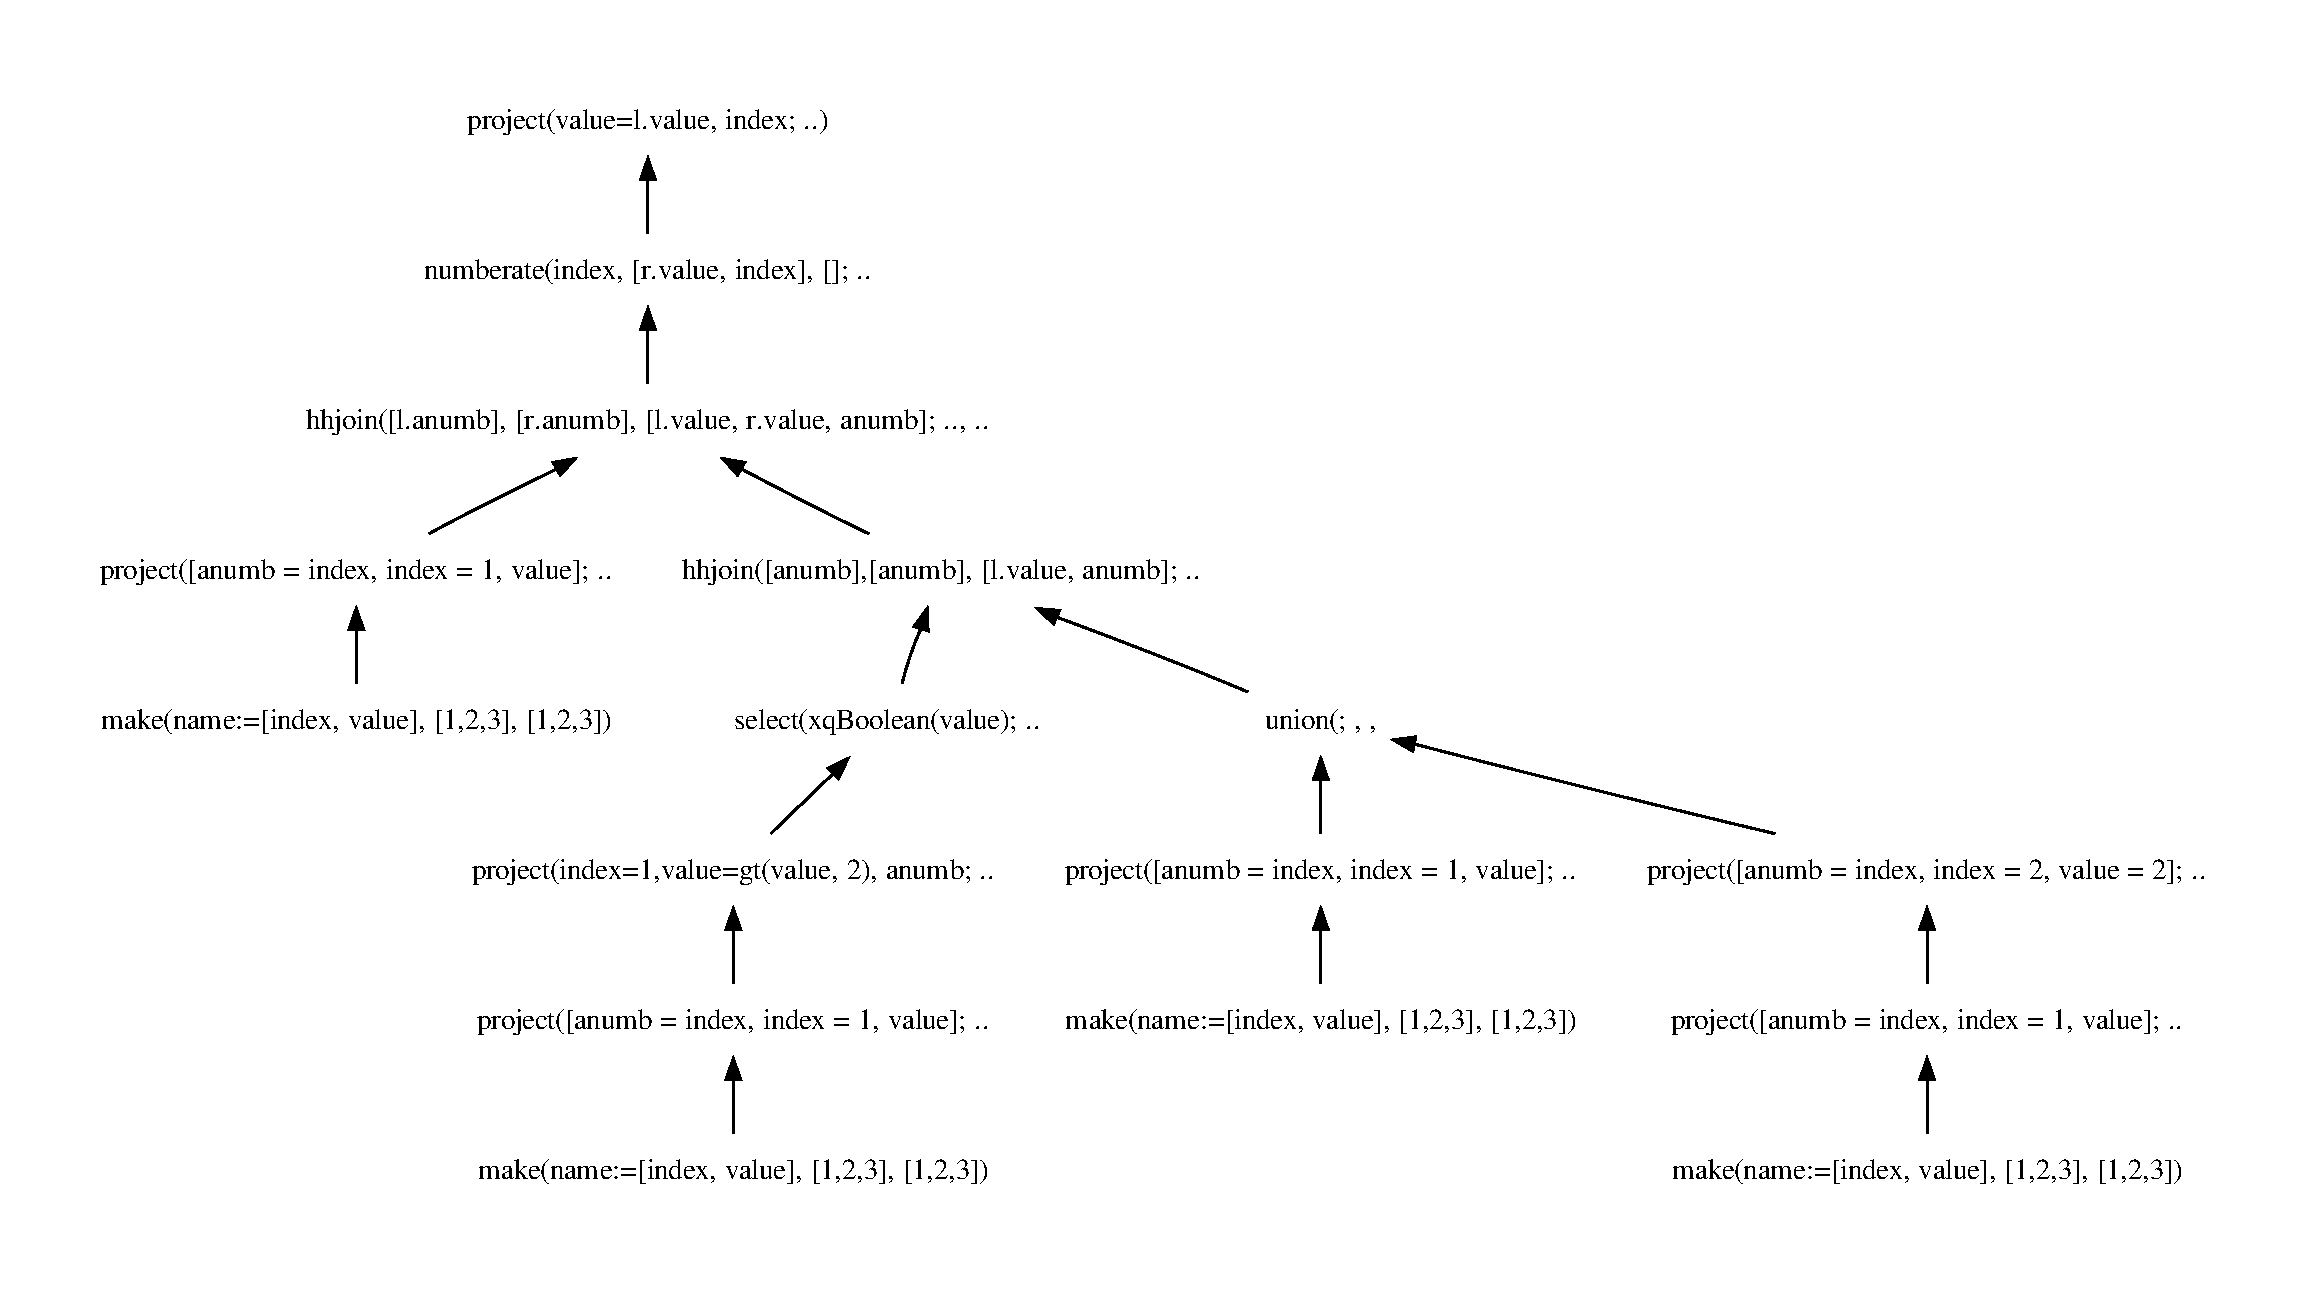
\includegraphics[width=1.0\textwidth]{img/graphs/ext_flwor}
  \caption{Complete translation of expression in figure
  \ref{fig:results:query_ext_flwor}}
  \label{fig:results:query_ext_flwor_result}
\end{center}
\end{figure}

The operator tree in figure \ref{fig:results:query_ext_flwor_result} can be
converted to the DAG seen in figure \ref{fig:results:query_ext_flwor_dag}.

\newpage

\begin{figure}[!htp]
\begin{center}
  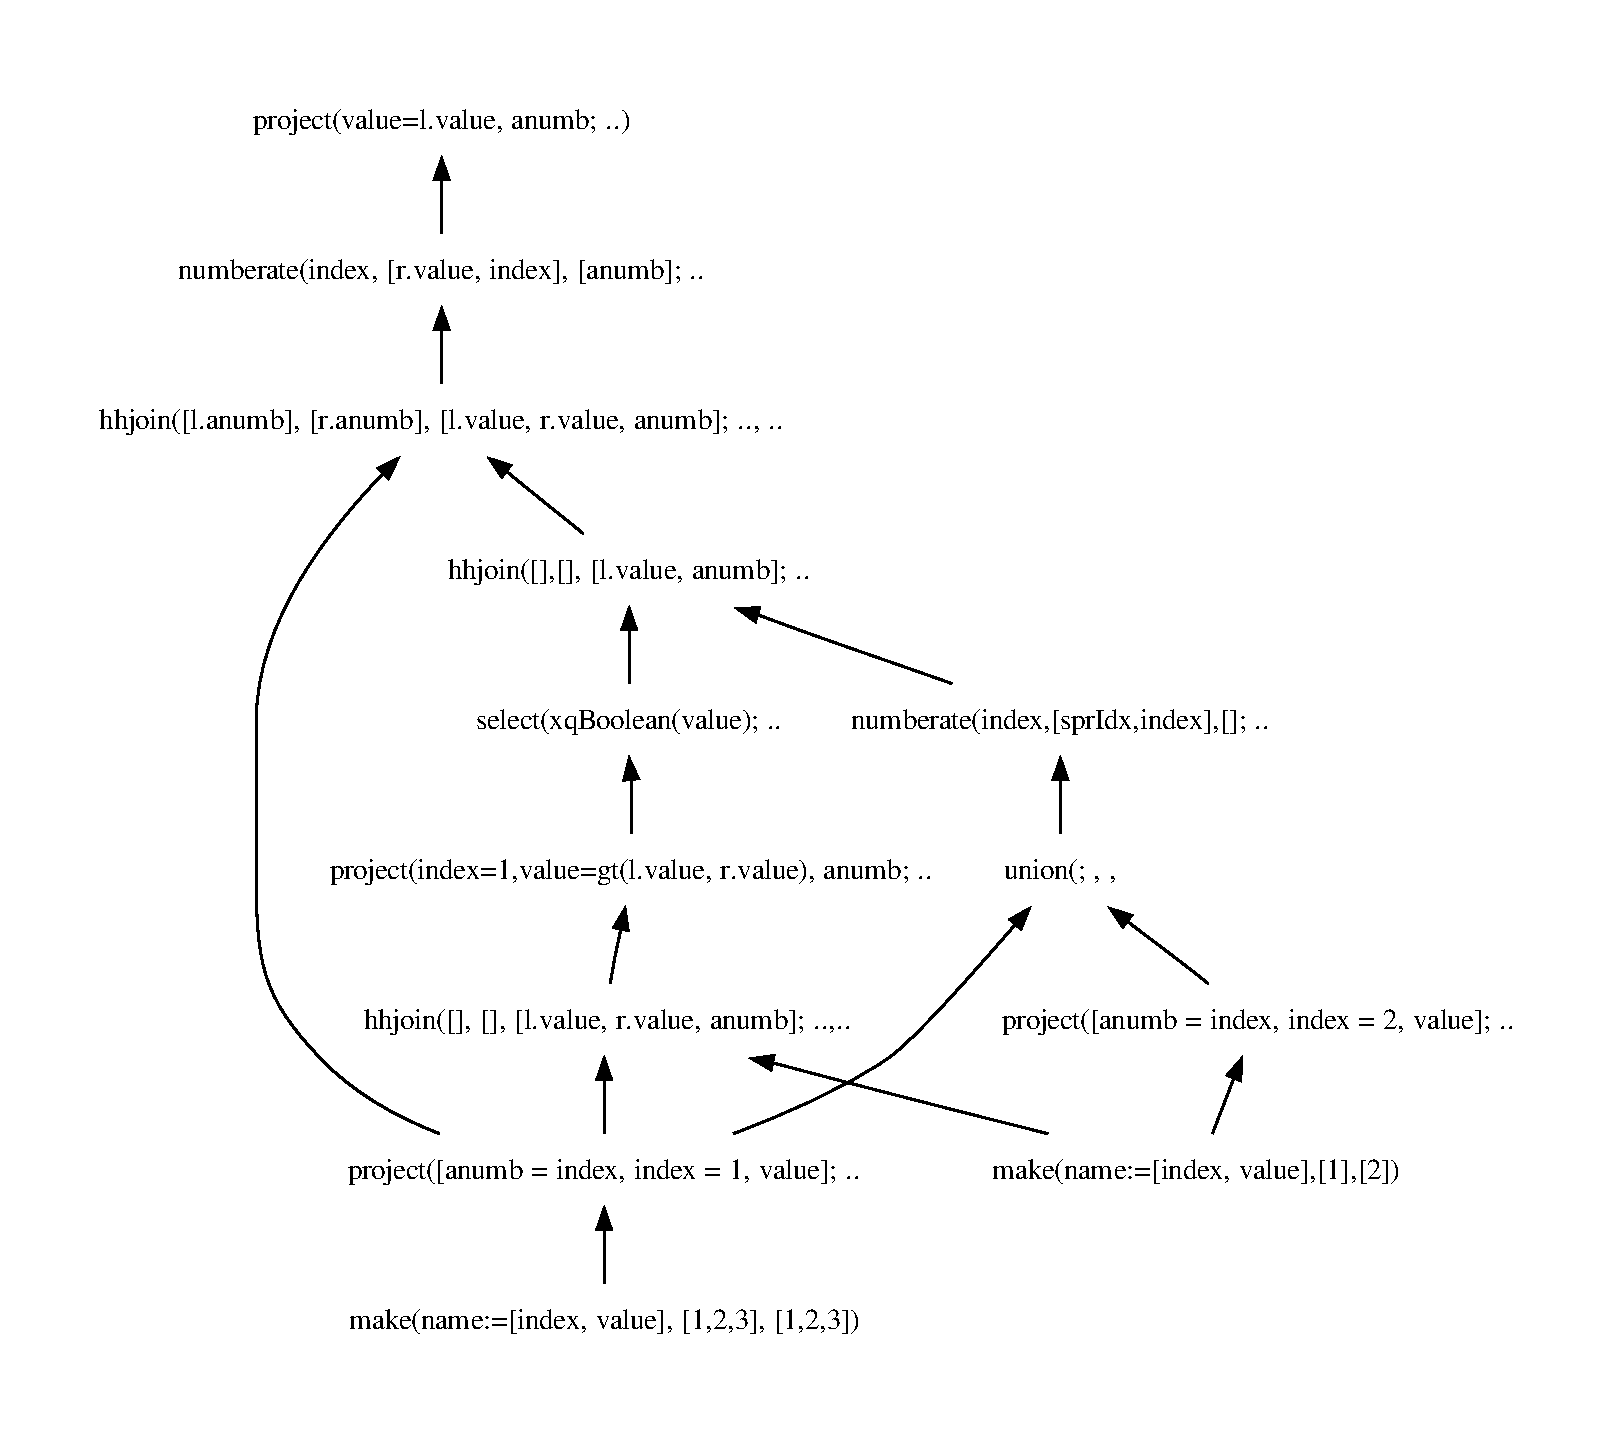
\includegraphics[width=1.0\textwidth]{img/graphs/ext_flwor_dag}
  \caption{DAG representation of operator tree in figure
  \ref{fig:results:query_ext_flwor_result}}
  \label{fig:results:query_ext_flwor_dag}
\end{center}
\end{figure}

\subsection{Path expression with predicate}
This example will illustrate the translation of a path expression with a predicate.

\subsubsection{Query premise}
\begin{figure}[!htp]
\begin{center}
\begin{Verbatim}
/a/b[@id eq 2] 
\end{Verbatim}
  \caption{Path expression with a predicate query premise}
  \label{fig:results:query_pathPred}
\end{center}
\end{figure}

\subsubsection{Translation process}
The translation process in its entirety is shown step by step in appendix
\ref{appendix:transl:pathPred}, page \pageref{appendix:transl:pathPred}.

\subsubsection{Result}
The result of the translation is shown in figure
\ref{fig:results:query_pathpred_result}.

\begin{figure}[!htp]
\begin{center}
  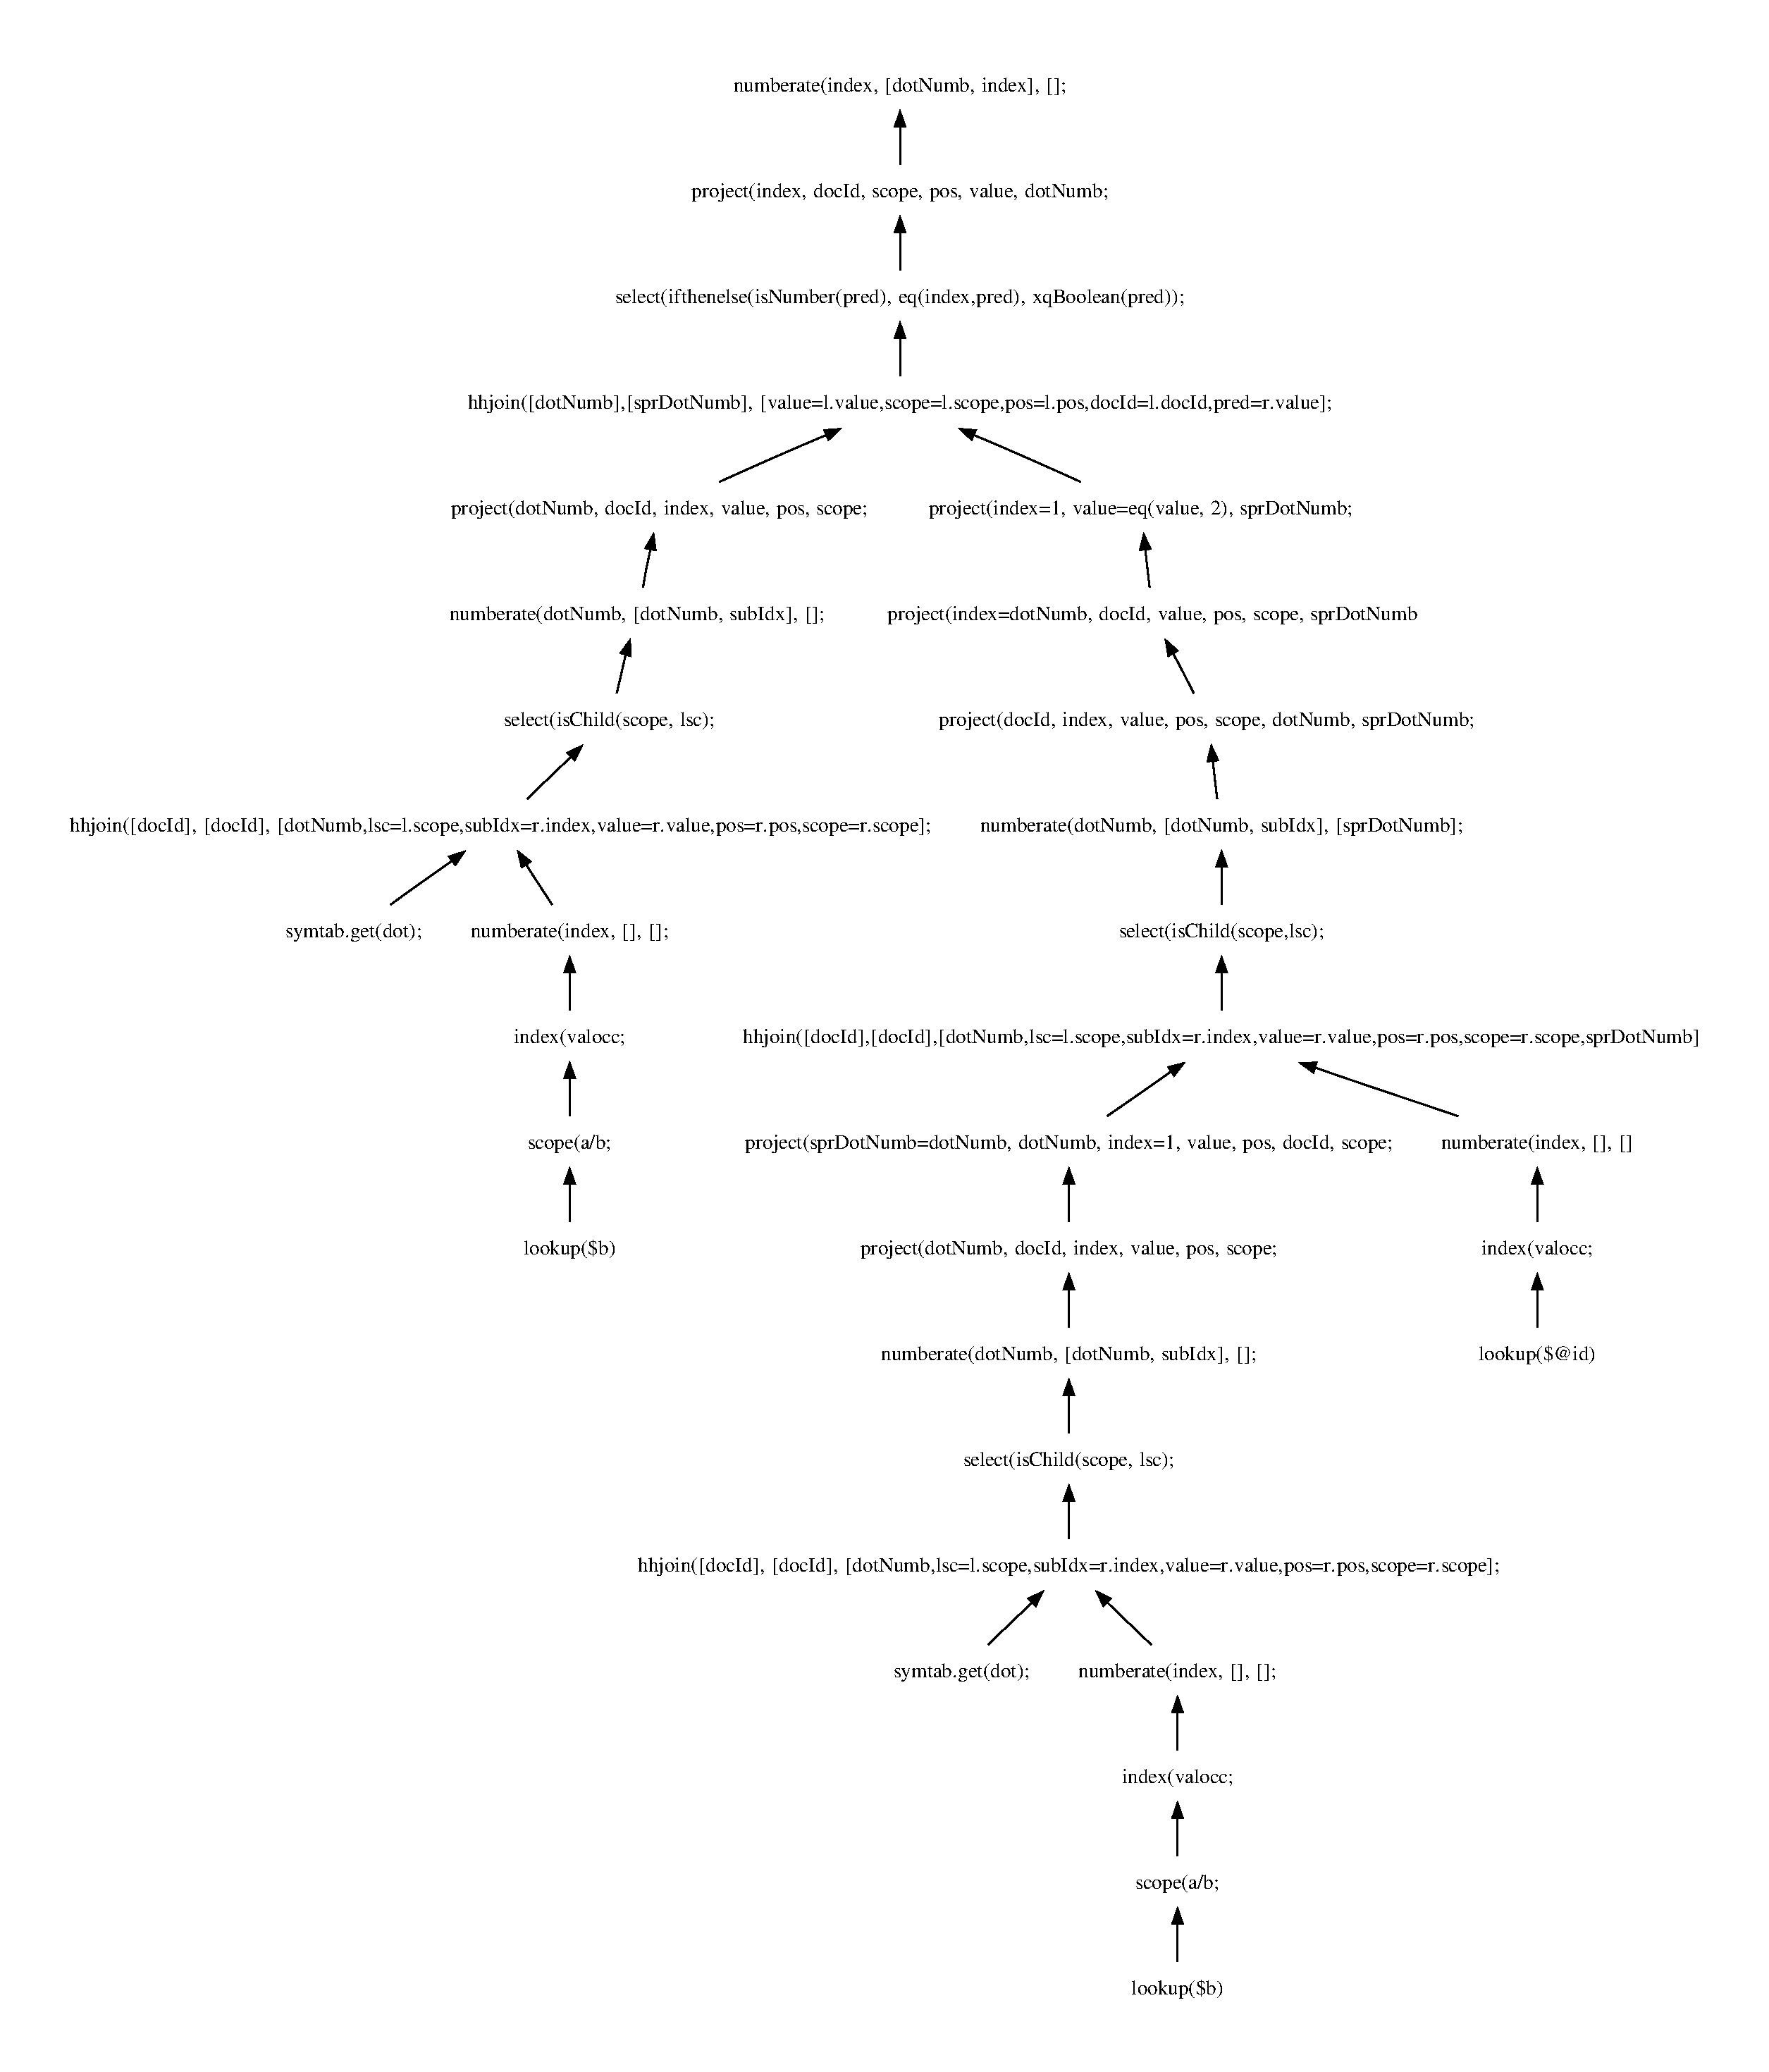
\includegraphics[width=1.0\textwidth]{img/graphs/TD_patExprPred}
  \caption{Complete translation of expression in figure
  \ref{fig:results:query_pathPred}}
  \label{fig:results:query_pathpred_result}
\end{center}
\end{figure}

The operator tree in figure \ref{fig:results:query_pathpred_result} can be
converted to the DAG seen in figure \ref{fig:results:query_pathpred_result_dag}.

\newpage

\begin{figure}[!htp]
\begin{center}
  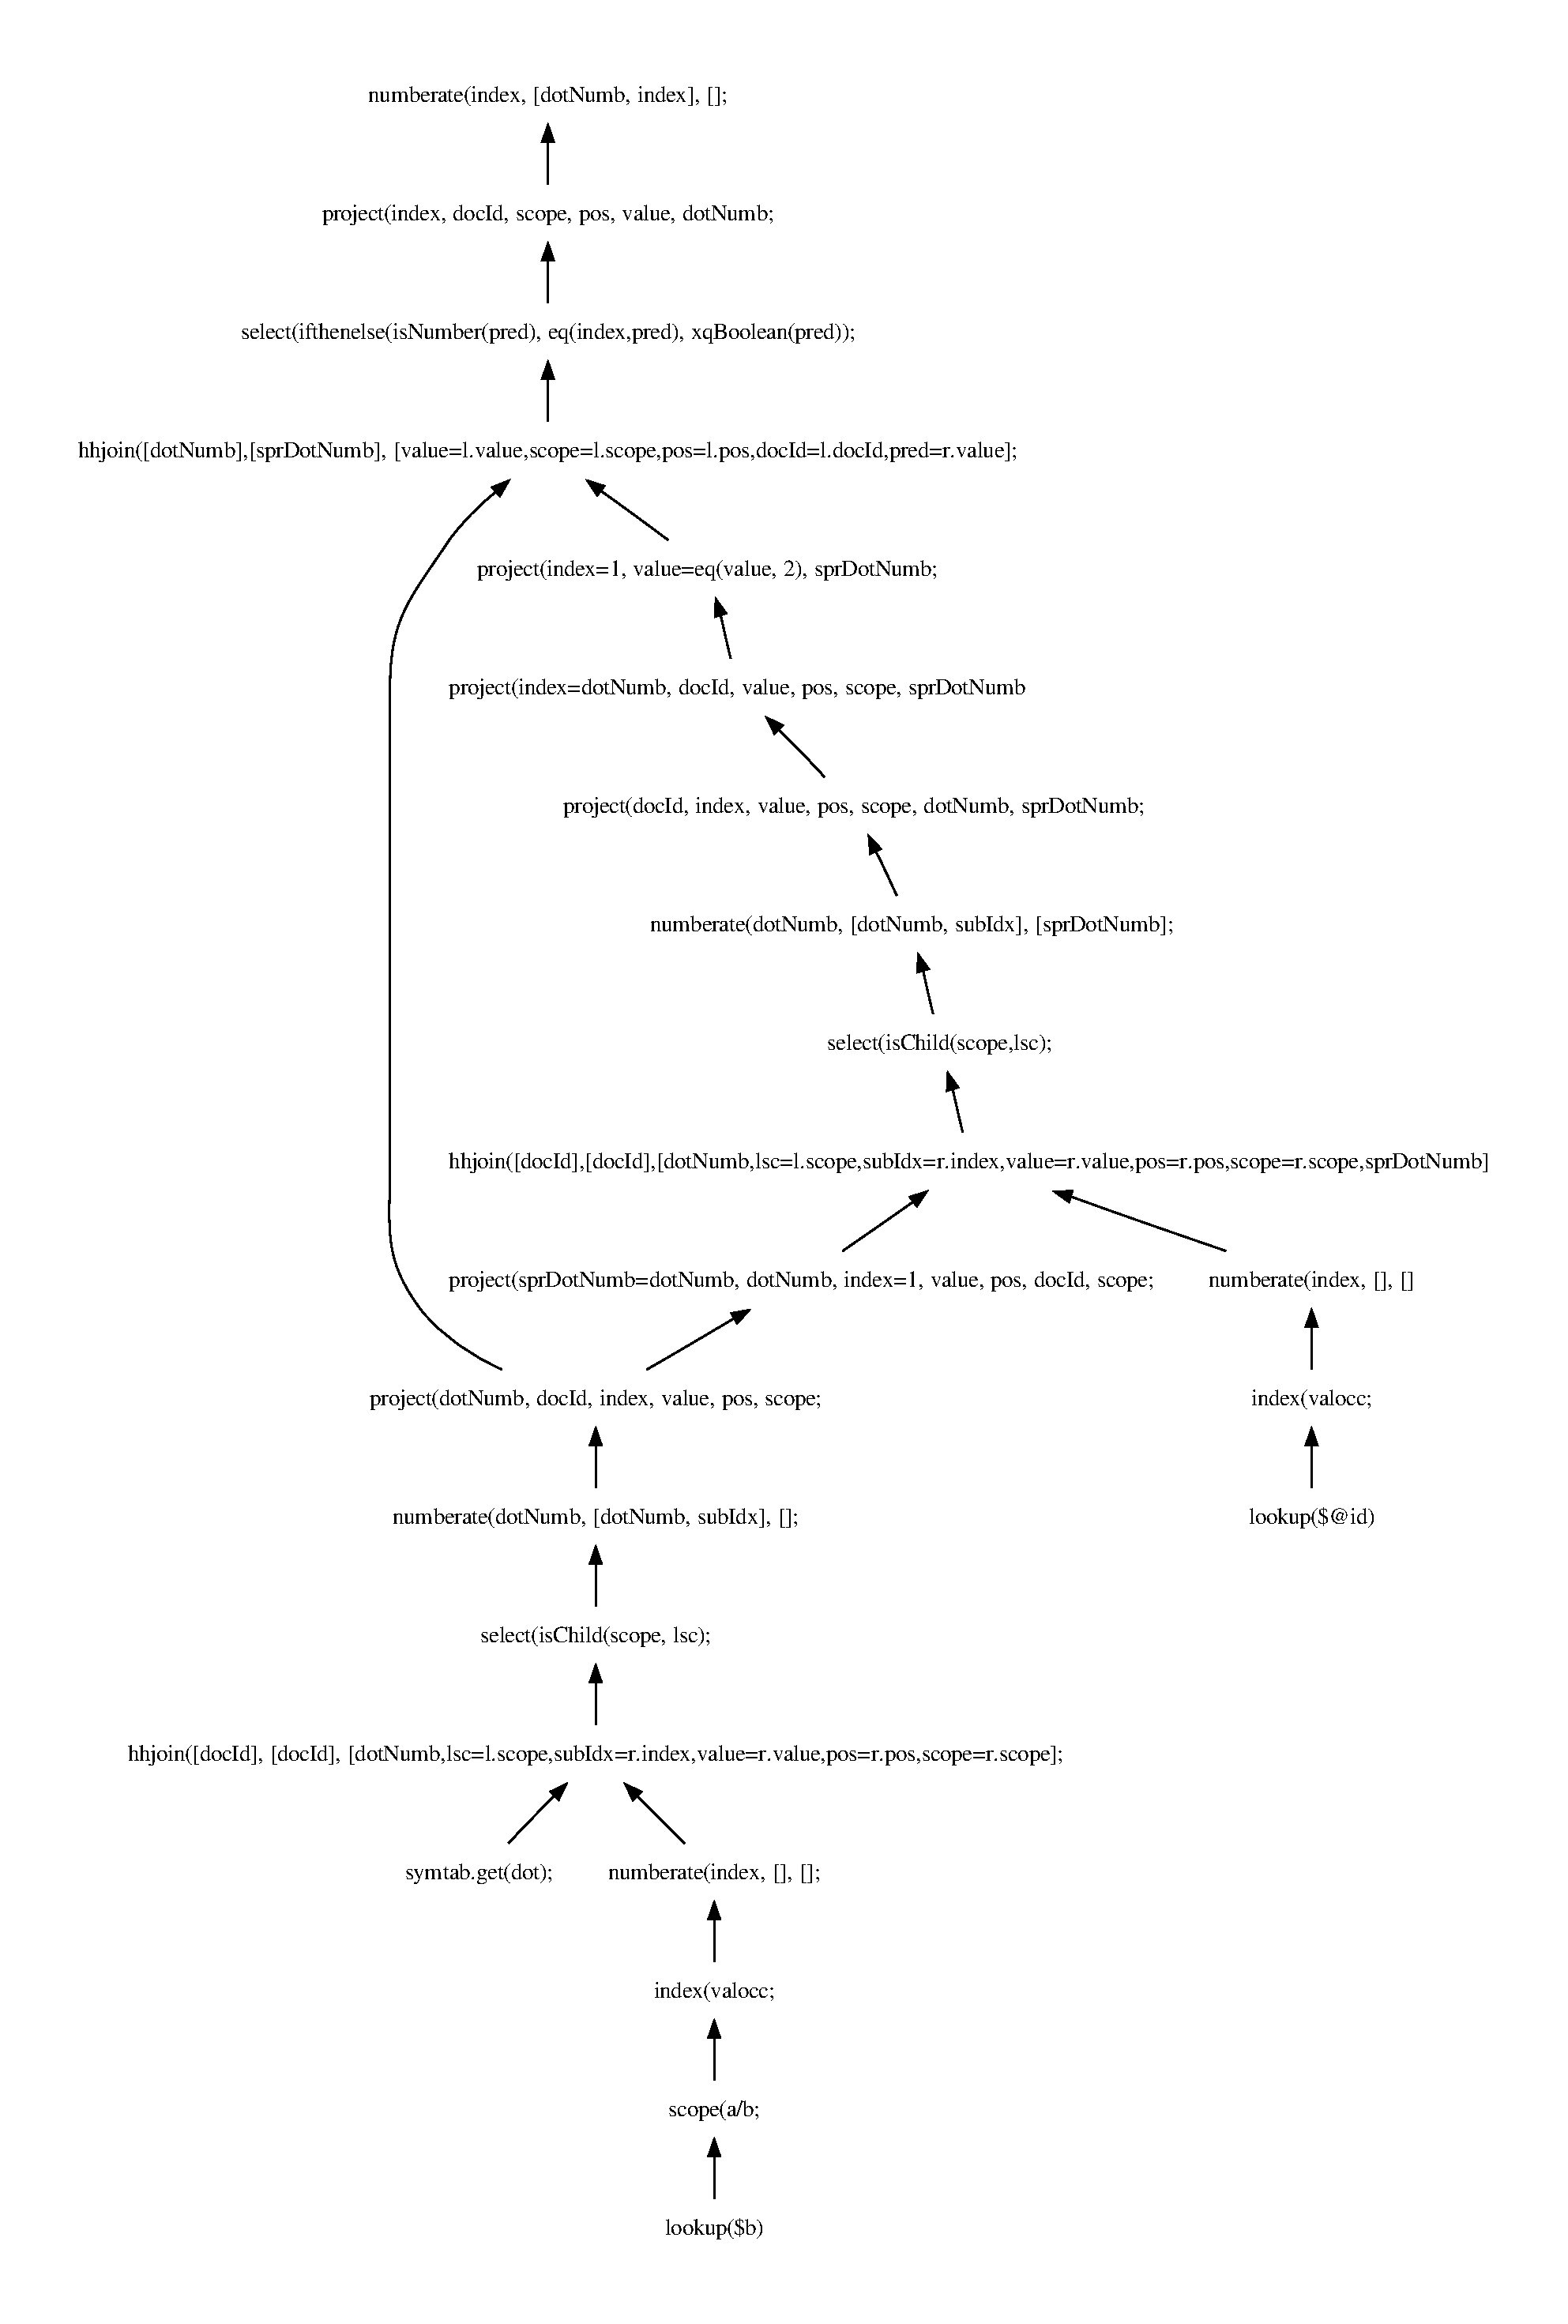
\includegraphics[width=1.0\textwidth]{img/graphs/TD_patExprPred_dag}
  \caption{DAG representation of operator tree in figure
  \ref{fig:results:query_pathpred_result}}
  \label{fig:results:query_pathpred_result_dag}
\end{center}
\end{figure}

\subsection{If-then-else}
\subsubsection{Query premise}
\begin{figure}[!htp]
\begin{center}
\begin{Verbatim}
for $a in (1,2,3) return
  if $a gt 2 then $a else 3
\end{Verbatim}
  \caption{If-then-else query premise}
  \label{fig:results:query_ifthenelse}
\end{center}
\end{figure}

\subsubsection{Translation process}
The translation process in its entirety is shown step by step in appendix
\ref{appendix:transl:ifthenelse}, page \pageref{appendix:transl:ifthenelse}.

\subsubsection{Result}
The result of the translation is shown in figure
\ref{fig:results:query_ifthenelse_result}.

\begin{figure}[!htp]
\begin{center}
  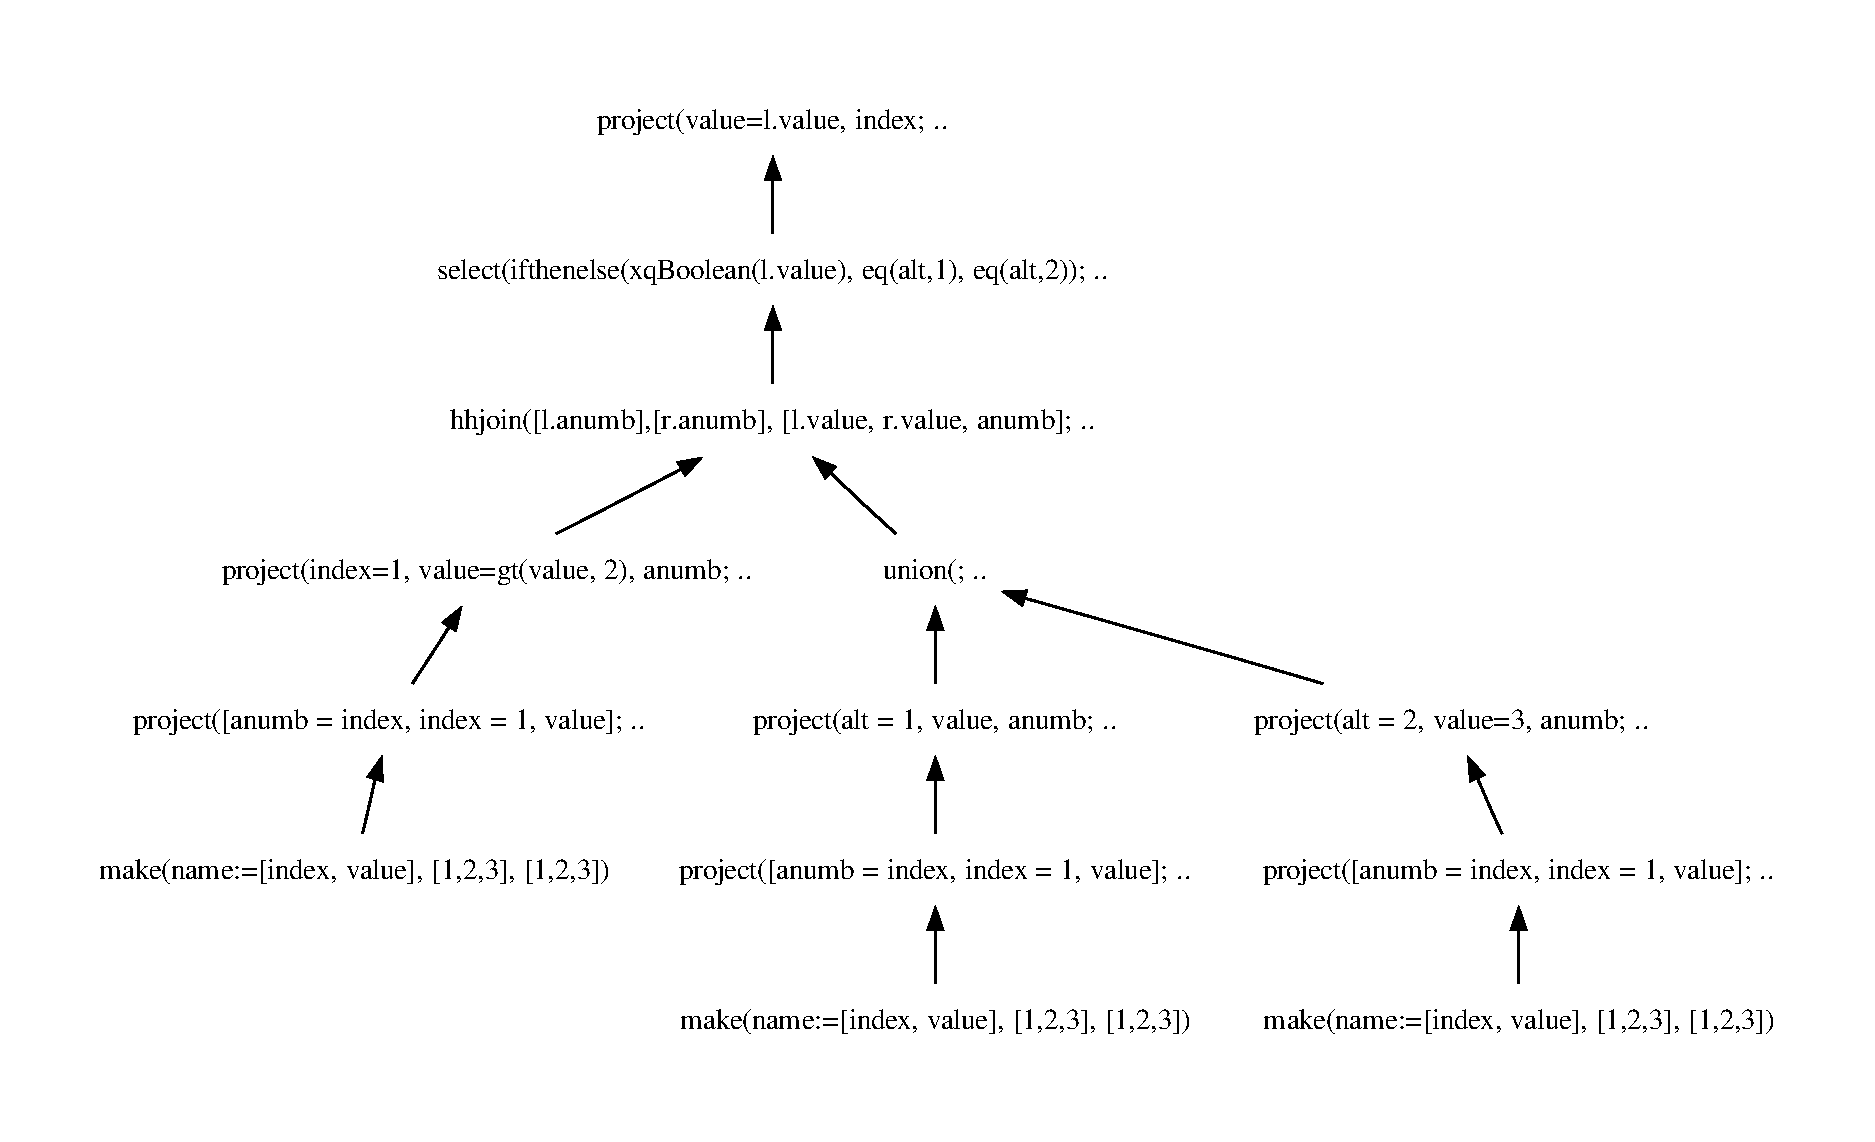
\includegraphics[width=1.0\textwidth]{img/graphs/ifthenelse}
  \caption{Complete translation of expression in figure
  \ref{fig:results:query_ifthenelse}}
  \label{fig:results:query_ifthenelse_result}
\end{center}
\end{figure}

The operator tree in figure \ref{fig:results:query_ifthenelse_result} can be
converted to the DAG seen in figure \ref{fig:results:query_ifthenelse_result_dag}.

\newpage

\begin{figure}[!htp]
\begin{center}
  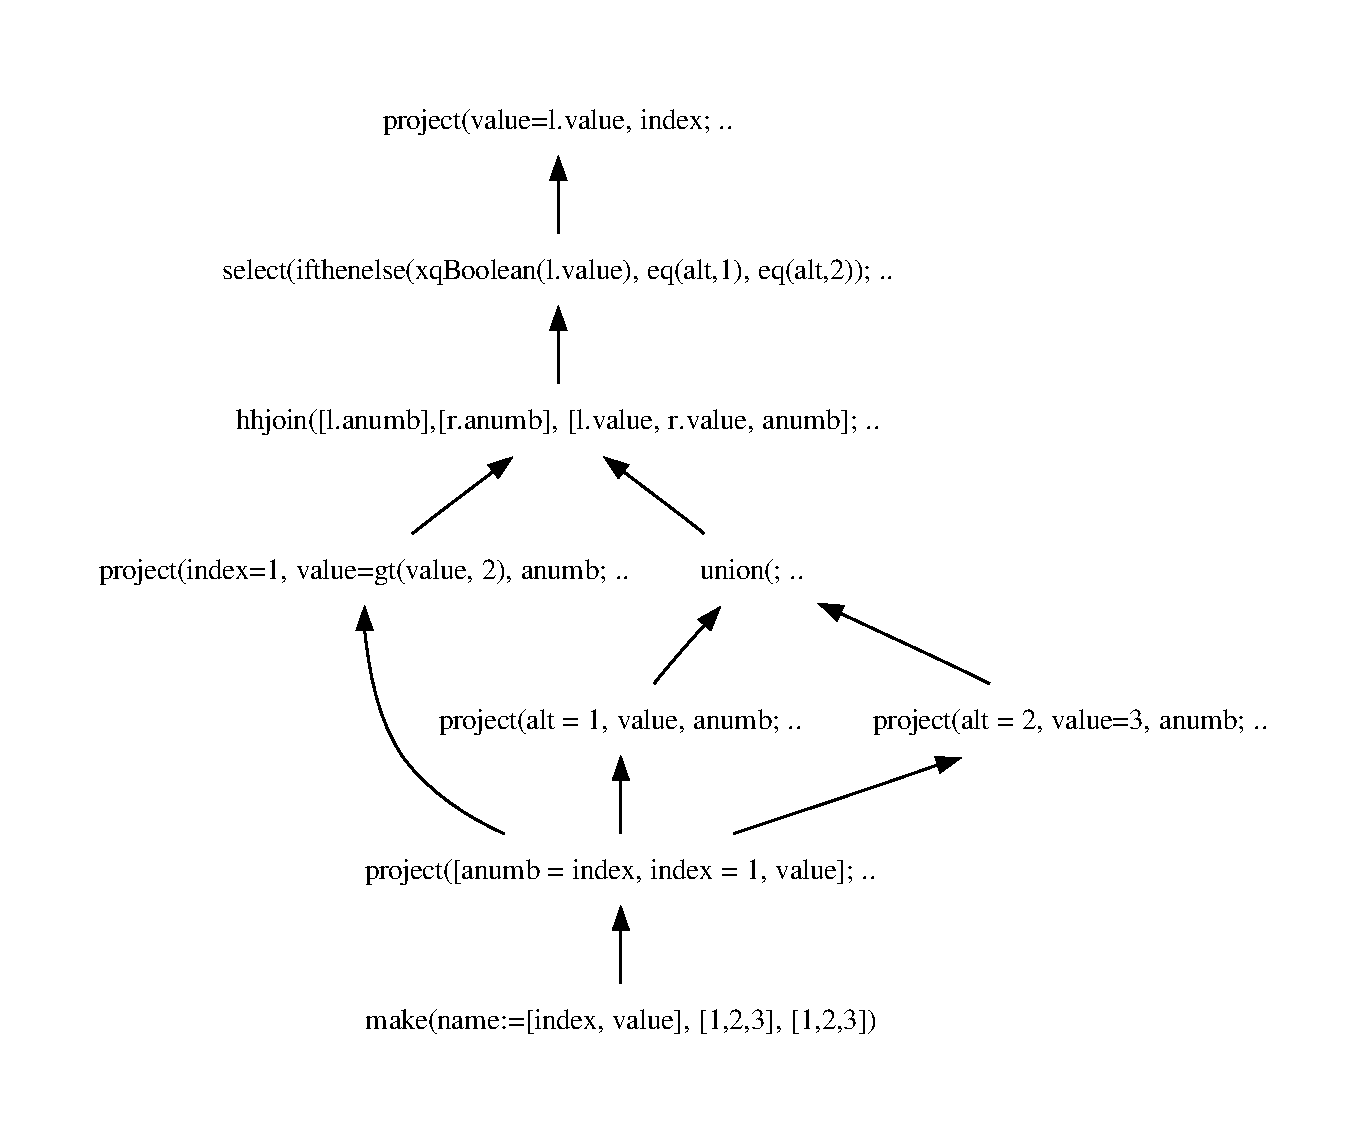
\includegraphics[width=1.0\textwidth]{img/graphs/ifthenelse_dag}
  \caption{DAG representation of operator tree in figure
  \ref{fig:results:query_ifthenelse_result}}
  \label{fig:results:query_ifthenelse_result_dag}
\end{center}
\end{figure}

\newpage

\section{Algebra Generated By Implementation}
\label{sect:result:implementation_algebra}
In this section, a collection of trivial queries are translated to relational
algebra using the implemented proof of concept described in chapter
\ref{chapter:implementation}. Naturally, this implementation also uses the
``Tainting Dependencies'' method, however the results from these translations
can also be used in a comparison with loop lifting.

\subsection{Trivial FLWOR}
\label{sect:results:algebra:generated:trivial_flwor}
\subsubsection{Query premise}
\begin{figure}[!htp]
\begin{center}
\begin{Verbatim}
for $a in (1,2,3) return $a
\end{Verbatim}
  \caption{Trivial FLWOR query premise}
  \label{fig:results:query_trivial_flwor}
\end{center}
\end{figure}

\subsubsection{Result}
\begin{figure}[!htp]
\begin{center}
  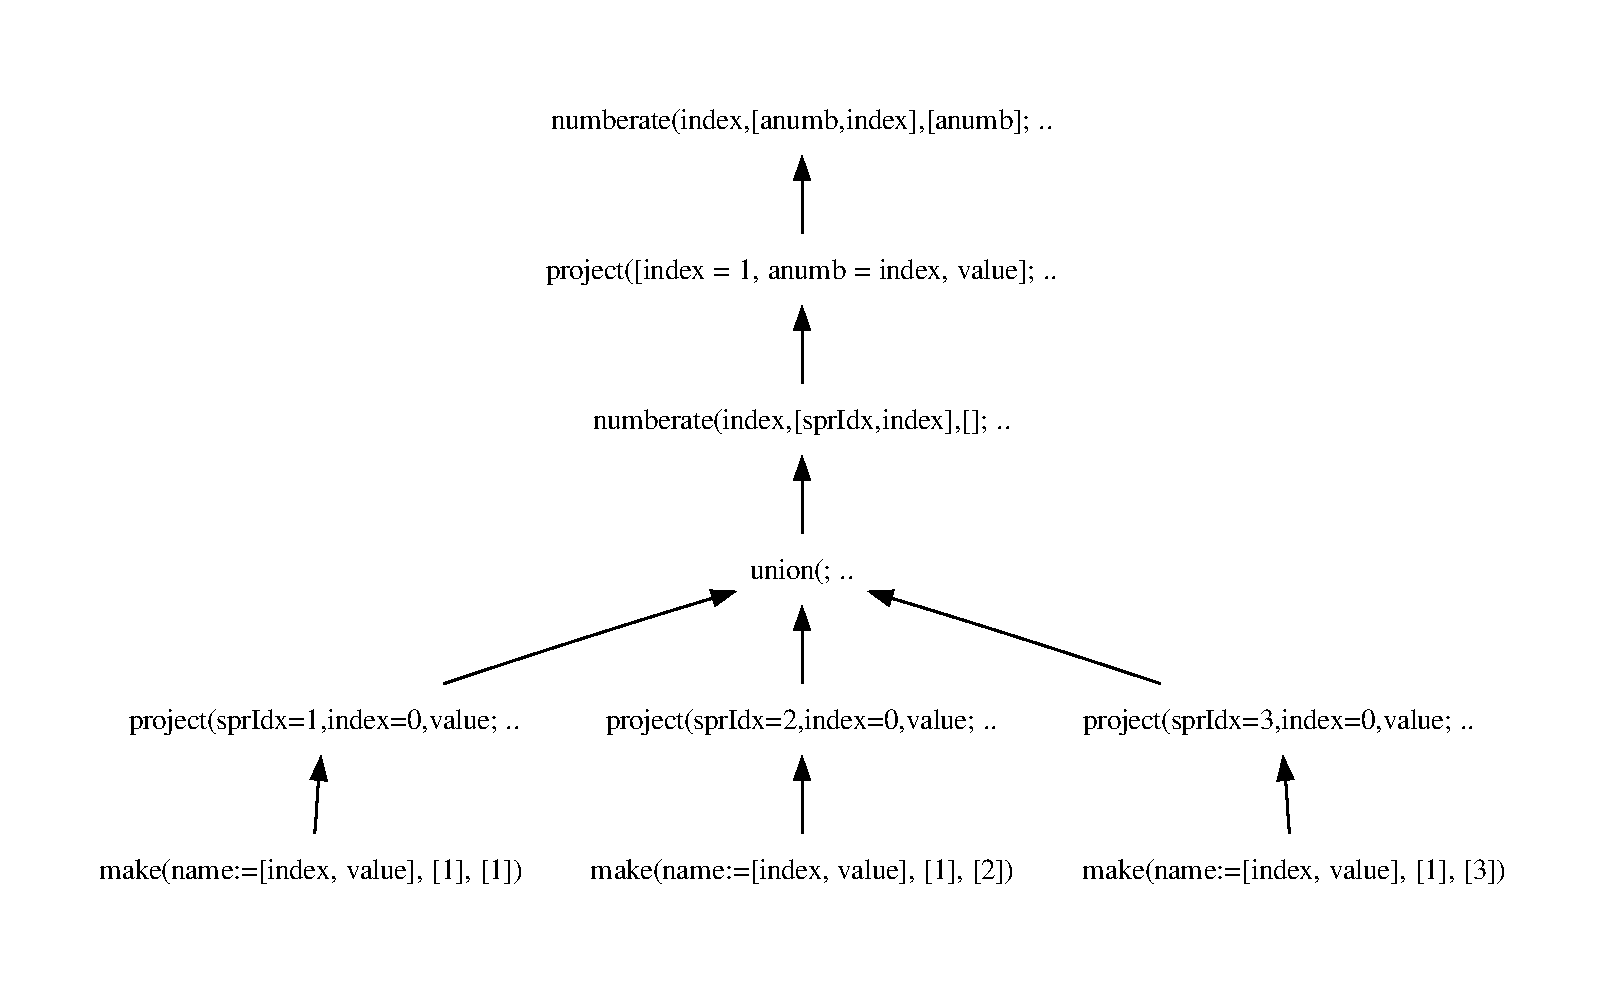
\includegraphics[width=1.0\textwidth]{img/graphs/td_impl_flwor_simple_xq_relalg} \caption{Complete translation of expression in figure
  \ref{fig:results:query_trivial_flwor}}
  \label{fig:results:query_trivial_flwor_result}
\end{center}
\end{figure}

\subsection{Complex FLWOR}
\label{sect:results:algebra:generated:complex_flwor}
\subsubsection{Query premise}
\begin{figure}[!htp]
\begin{center}
\begin{Verbatim}
for $a in (1,2) return (3, for $b in (4,5) return ($a, $b, 6))
\end{Verbatim}
  \caption{Complex FLWOR query premise}
  \label{fig:results:query_complex_flwor}
\end{center}
\end{figure}

\subsubsection{Result}
\begin{figure}[!htp]
\begin{center}
  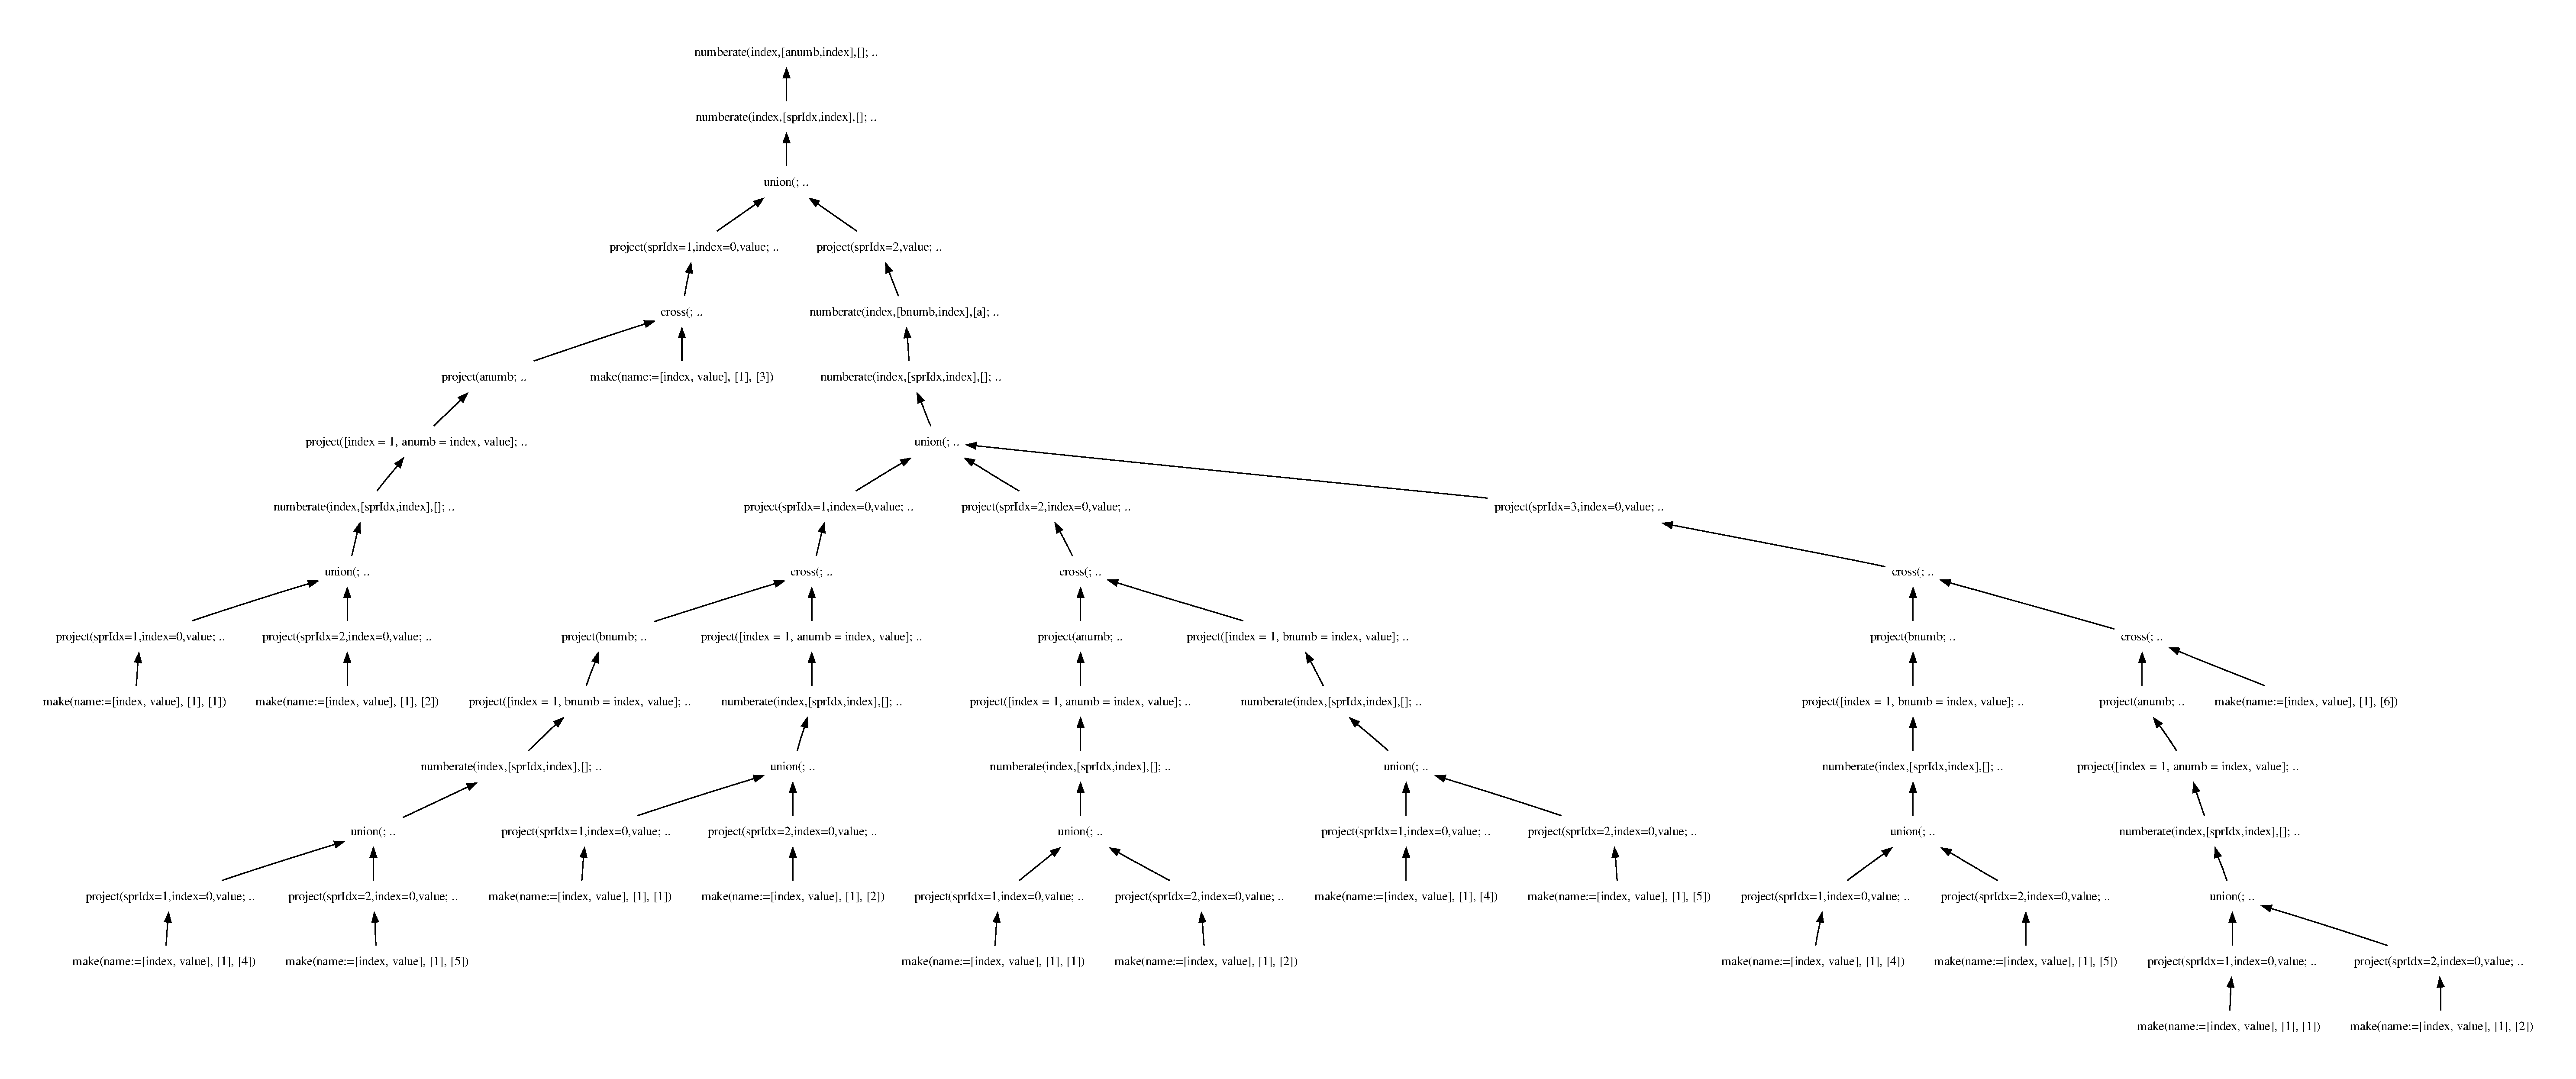
\includegraphics[angle=90,height=0.7\textheight]{img/graphs/td_impl_flwor_complex_xq_relalg} \caption{Complete
  translation of expression in figure
  \ref{fig:results:query_complex_flwor}}
  \label{fig:results:query_complex_flwor_result}
\end{center}
\end{figure}


The algebra tree in figure \ref{fig:results:query_complex_flwor_result} can
be converted to the DAG in figure
\ref{fig:results:query_complex_flwor_result_dag}

\begin{figure}[!htp]
\begin{center}
  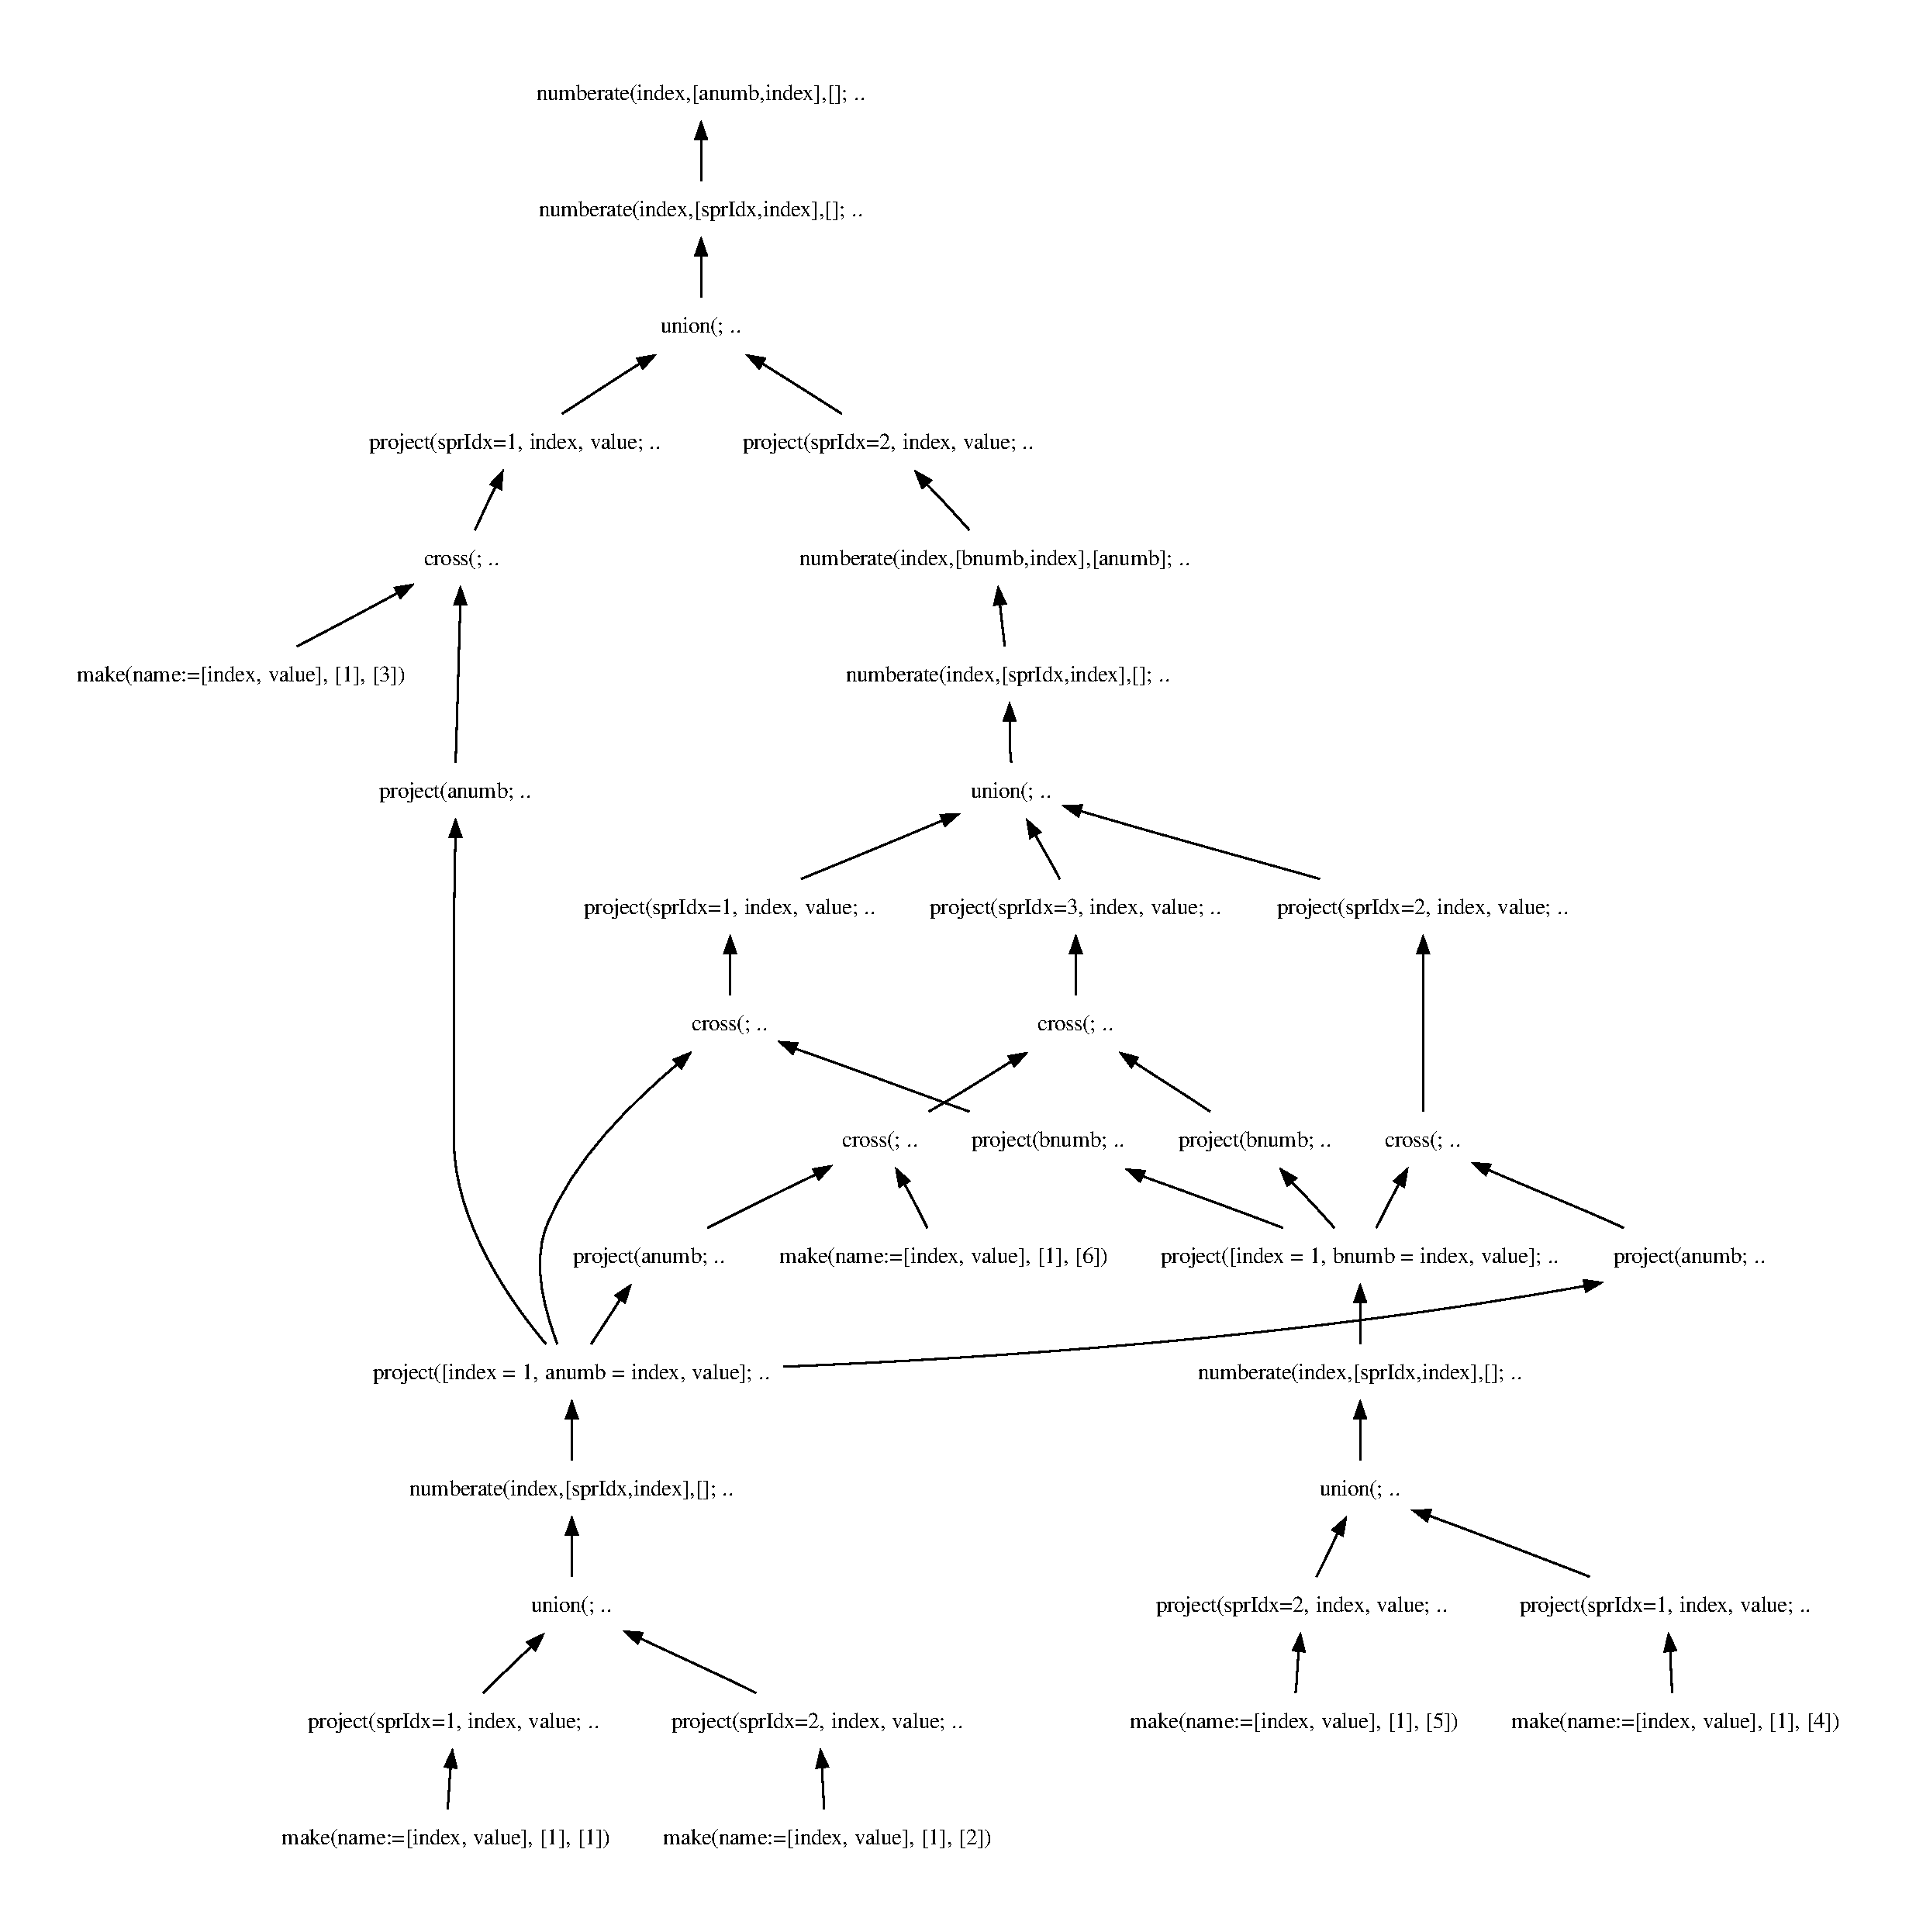
\includegraphics[width=1.0\textwidth]{img/graphs/td_impl_flwor_complex_xq_relalg_dag}
  \caption{Complete translation of expression in figure
  \ref{fig:results:query_complex_flwor} converted to a DAG}
  \label{fig:results:query_complex_flwor_result_dag}
\end{center}
\end{figure}
\newpage

\subsection{FLWOR with conditional}
\label{sect:results:algebra:generated:conditional_flwor}
\subsubsection{Query premise}
\begin{figure}[!htp]
\begin{center}
\begin{Verbatim}
for $a in (10,20) return if ($a > 15) then $a else 15
\end{Verbatim}
  \caption{Conditional FLWOR query premise}
  \label{fig:results:query_conditional_flwor}
\end{center}
\end{figure}

\subsubsection{Result}
\begin{figure}[!htp]
\begin{center}
  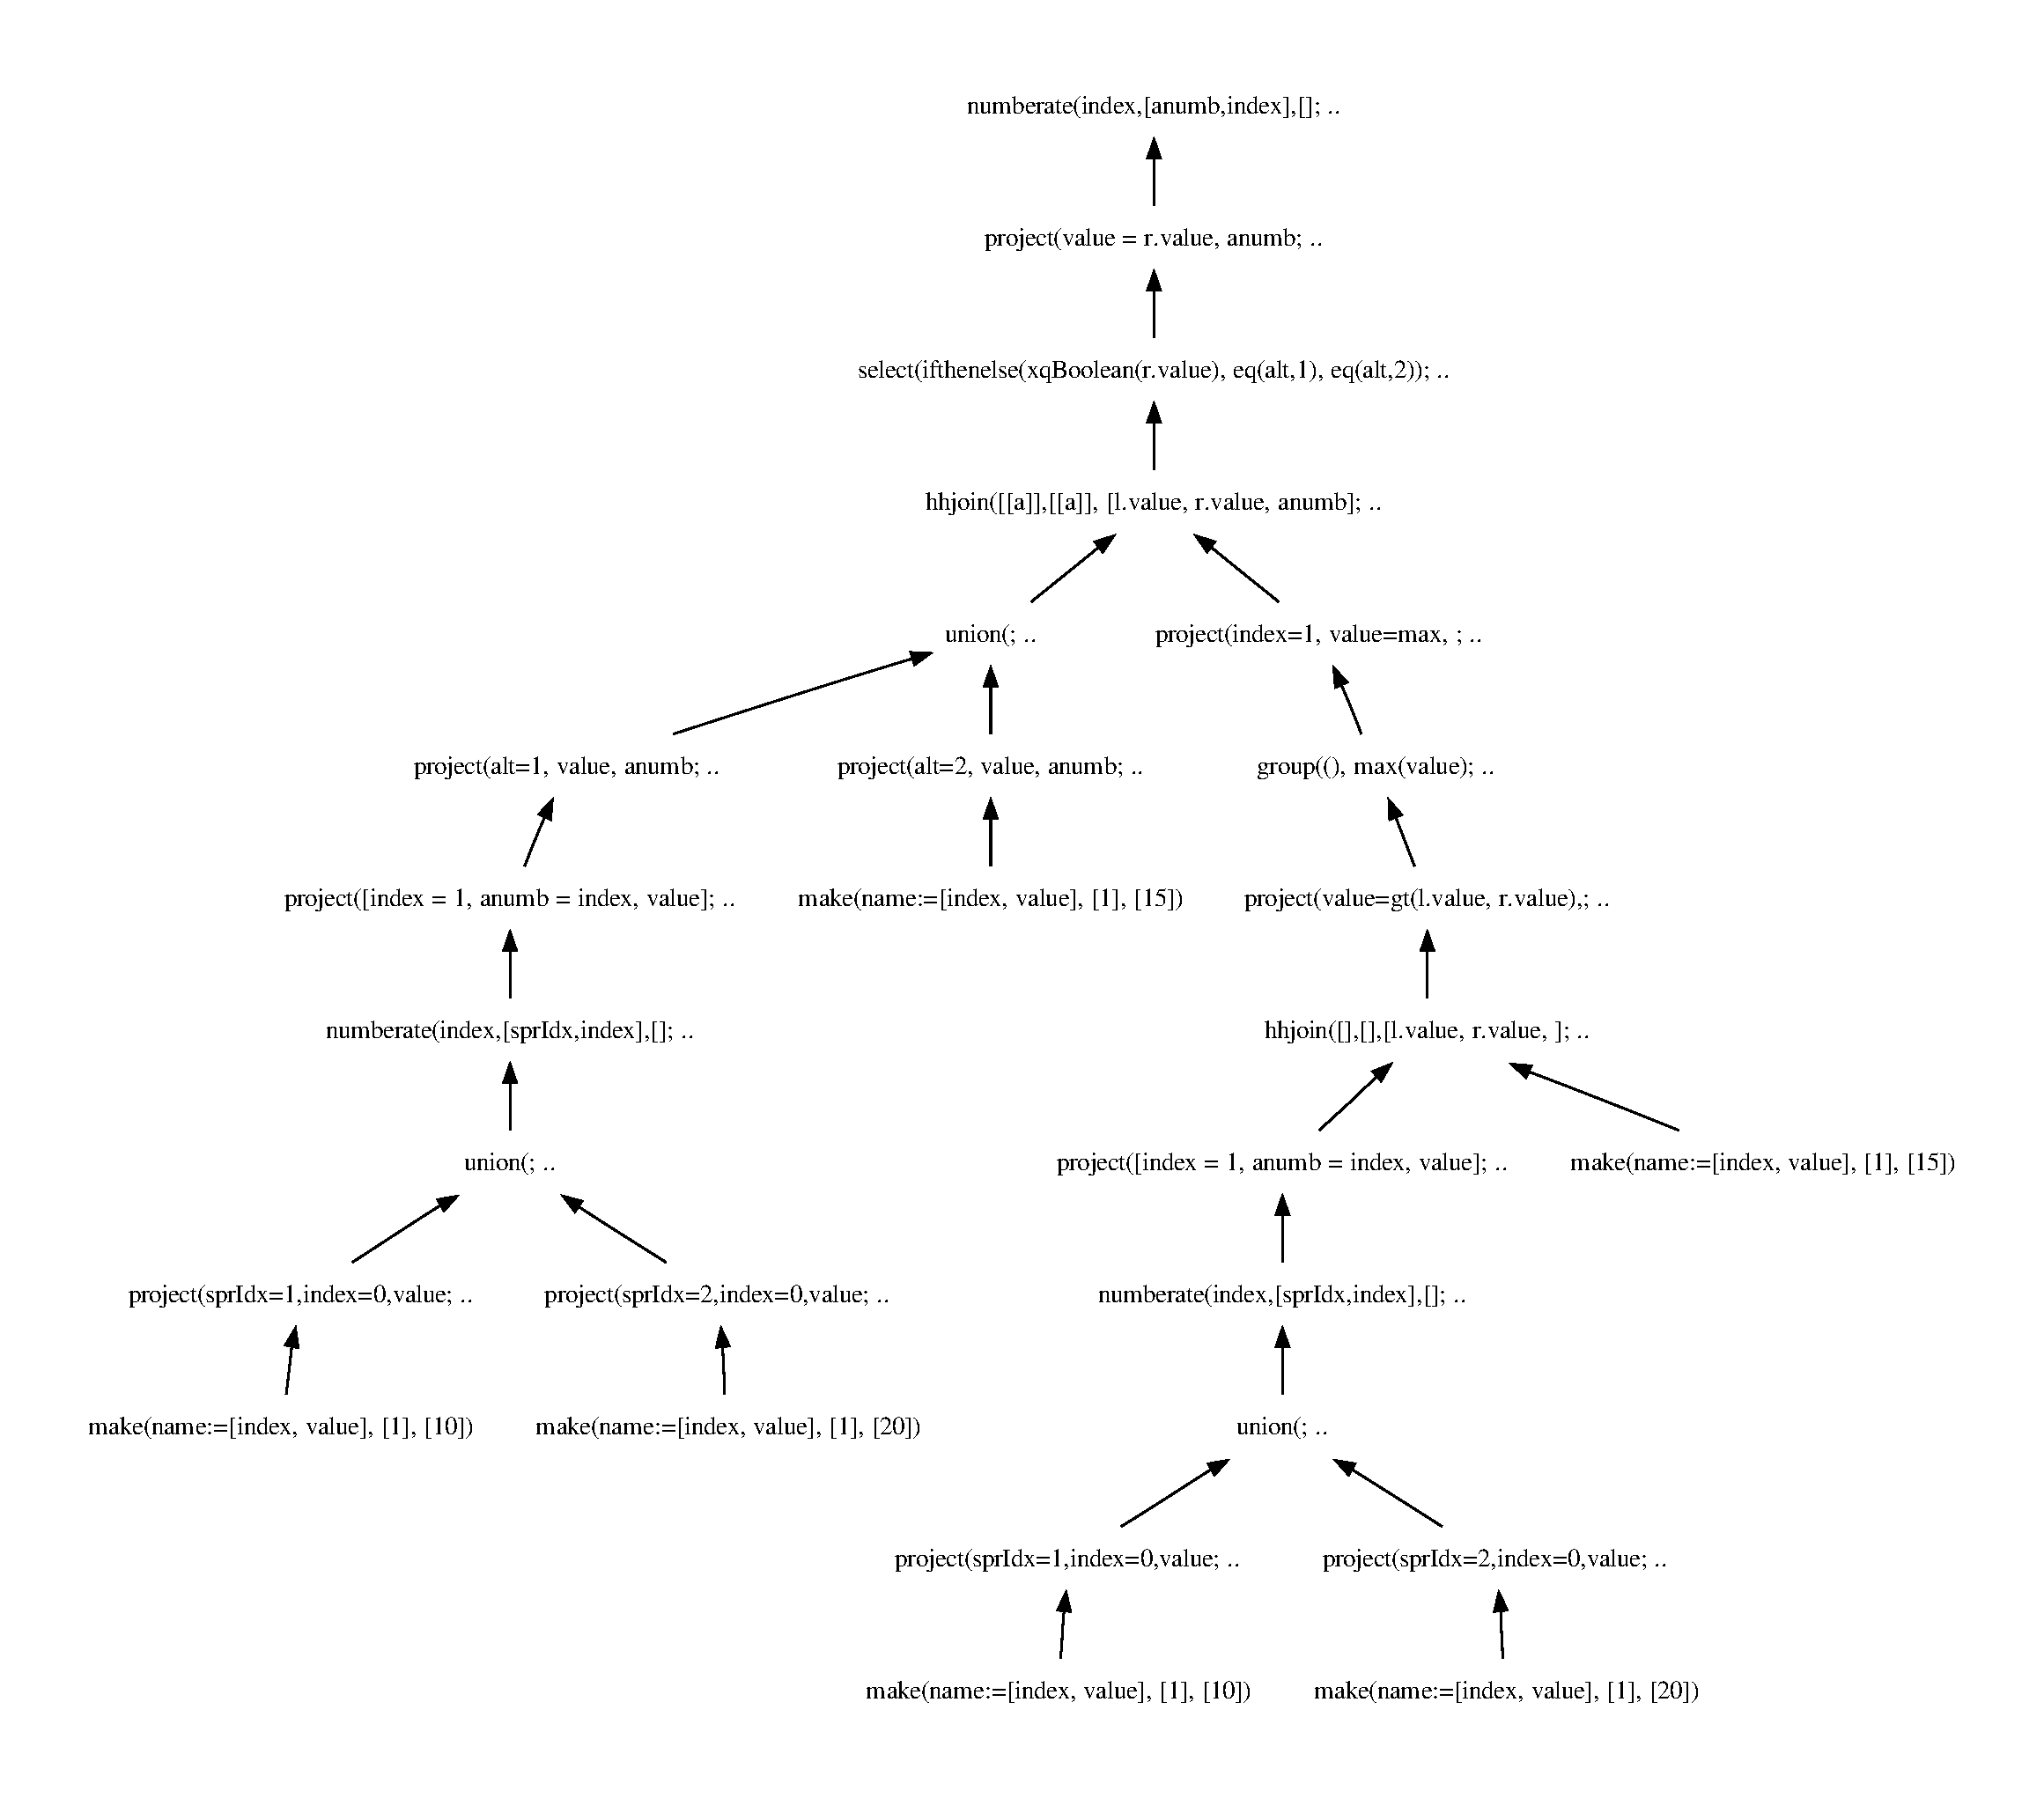
\includegraphics[width=1.0\textwidth]{img/graphs/td_impl_flwor_ifthenelse_xq_relalg}
  \caption{Complete translation of expression in figure
  \ref{fig:results:query_conditional_flwor}}
  \label{fig:results:query_conditional_flwor_result}
\end{center}
\end{figure}

The algebra tree in figure \ref{fig:results:query_conditional_flwor_result} can
be converted to the DAG in figure
\ref{fig:results:query_conditional_flwor_result_dag}

\newpage
\begin{figure}[!htp]
\begin{center} 
  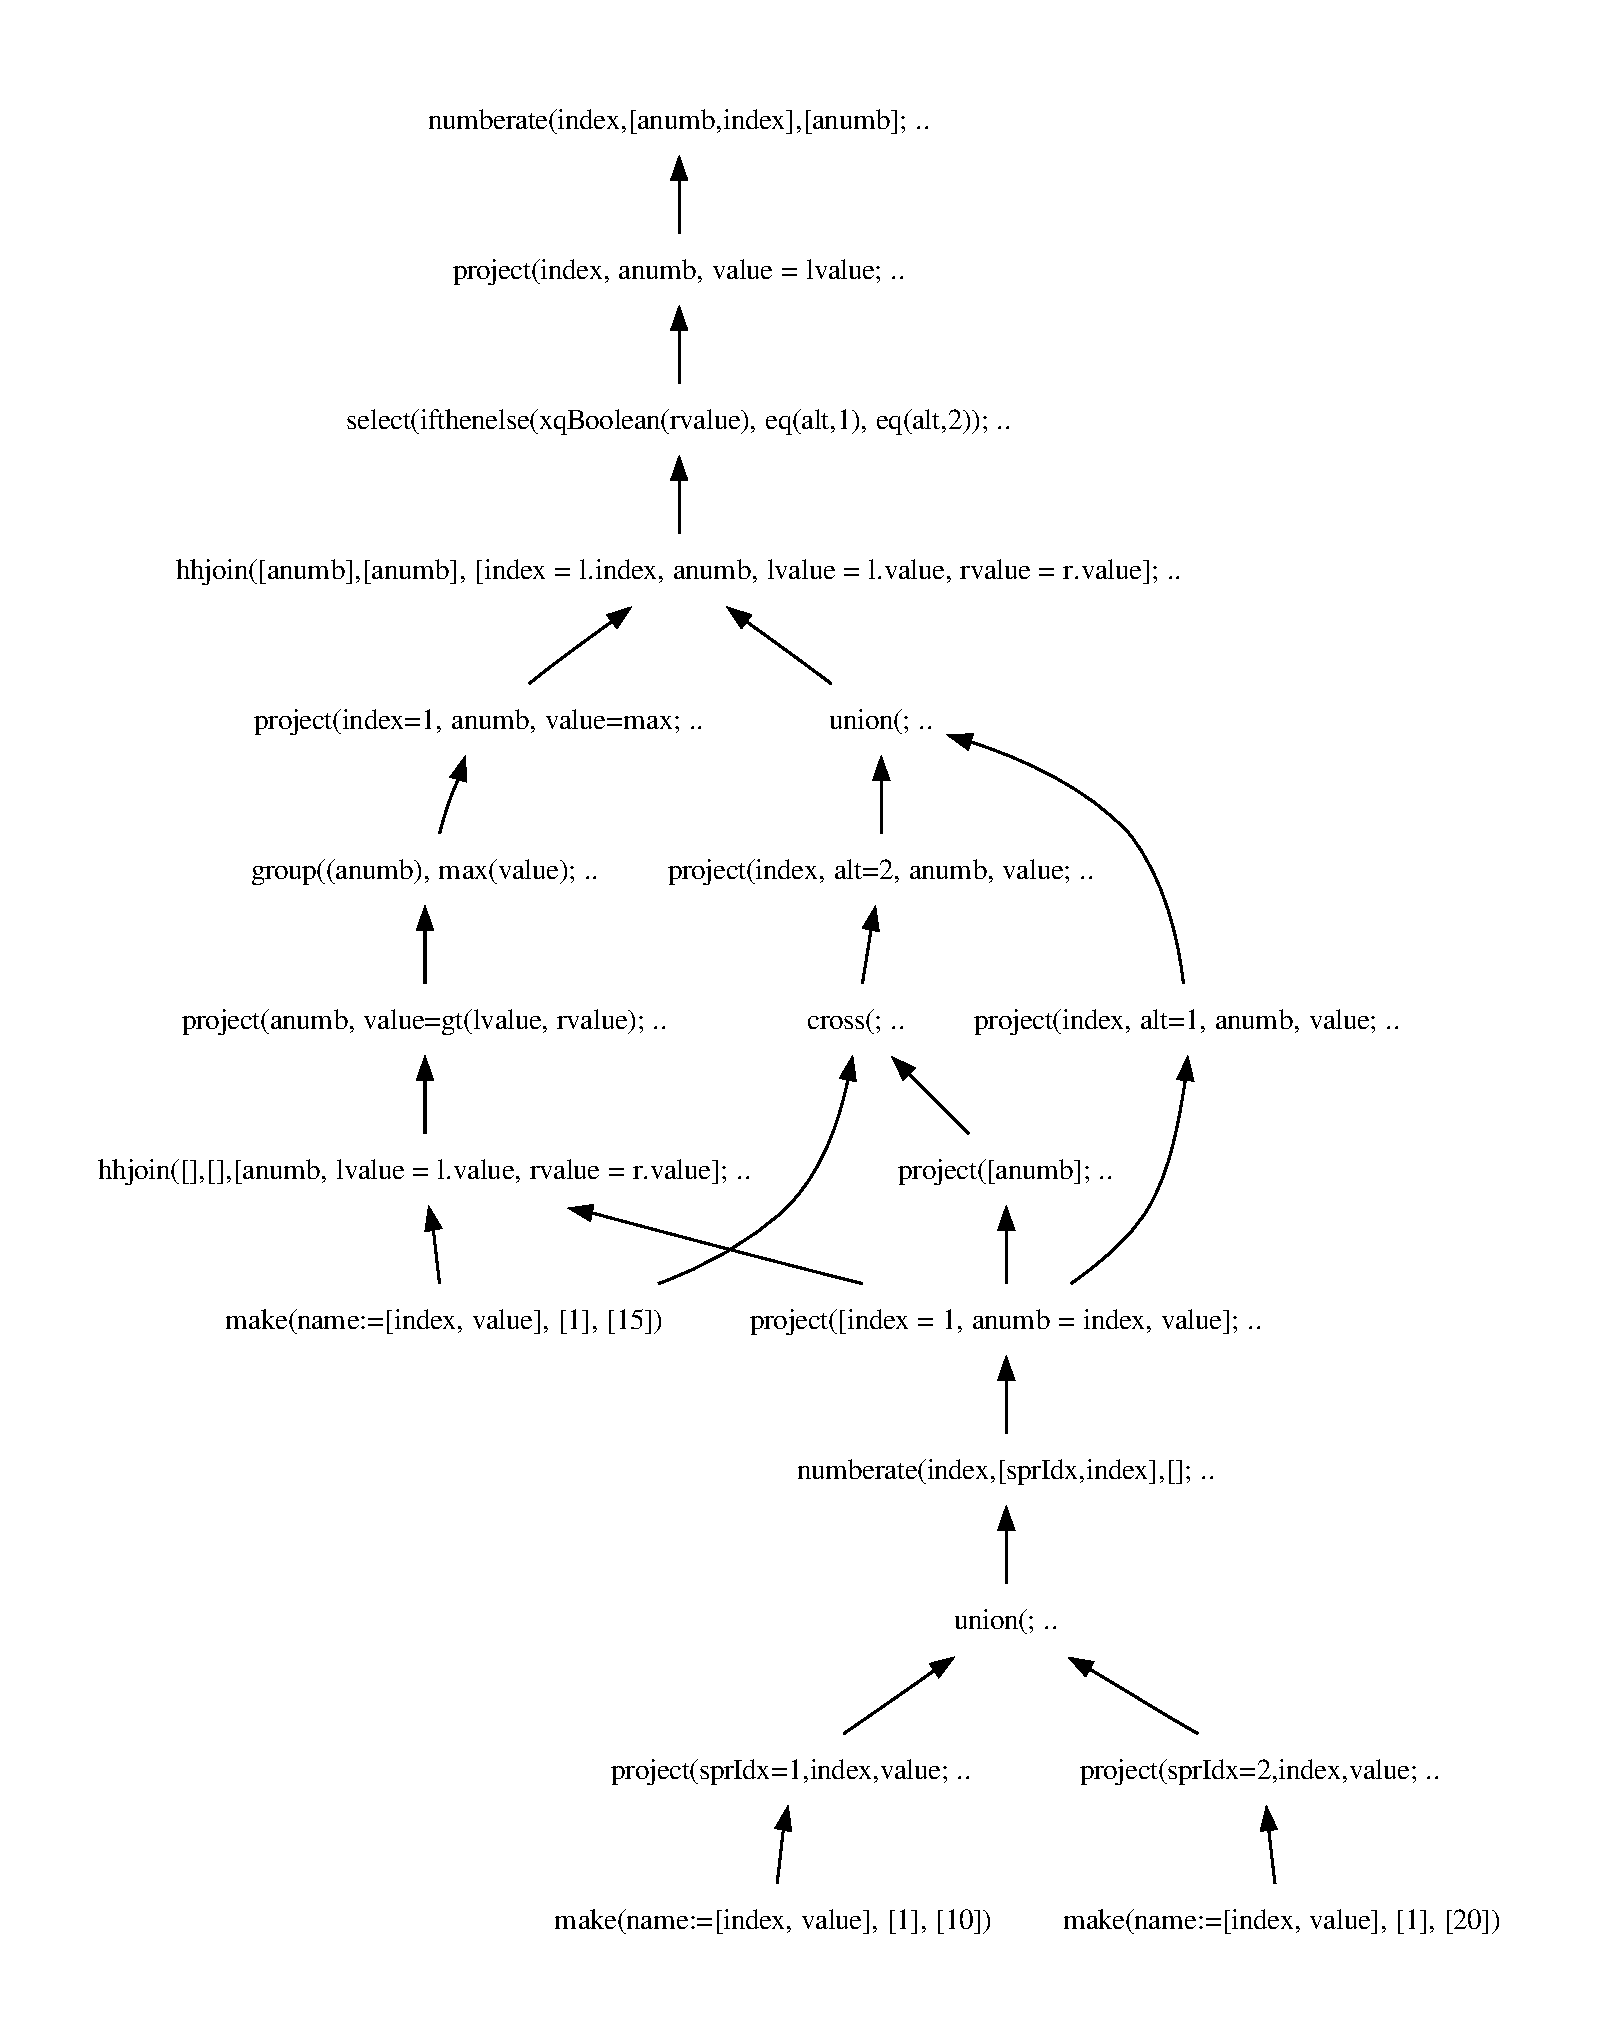
\includegraphics[width=1.0\textwidth]{img/graphs/td_impl_flwor_ifthenelse_xq_relalg_dag}
  \caption{Complete translation of expression in figure
  \ref{fig:results:query_conditional_flwor} converted to a DAG}
  \label{fig:results:query_conditional_flwor_result_dag}
\end{center}
\end{figure}
\section{Comparison}
\label{sect:results:comparison}
\subsection{Assumptions}
This comparison must be seen in the context of a number of assumptions
about the systems being compared. With regards to fairness, it is important to
note that the algebra trees generated by Pathfinder may have been
optimised (to which the exact extent is not known), while the algebra trees
generated by the prototype developed throughout this project \emph{does not apply any optimalisations} at all. The
optimalisations applied by Pathfinder are noted
in \cite{pathfinder_purelyRelational}.

Some important effects on the Pathfinder algebra tree from these
optimalisations are:
\begin{itemize}
  \item The cartesian products between a loop relation and a constant
  subexpression are transformed into projections
  \item The custom operator \textsf{attach} is roughly a simpler equivalent to
  the \textsf{make()} operator in MQL (see section \ref{sect:method:mql}, page
  \pageref{sect:method:mql})
\end{itemize}
TODO: noe mer her?

\newpage
\subsection{DAG comparison}
Note that the readability for these DAG comparisons are not essential --
however, links to large-scale versions of these diagrams are noted in appendix
\ref{appendix:links_and_resources}.

\begin{figure}[!h]
	\centering
	\mbox{
		\subfigure[Pathfinder/MonetDB]{		
			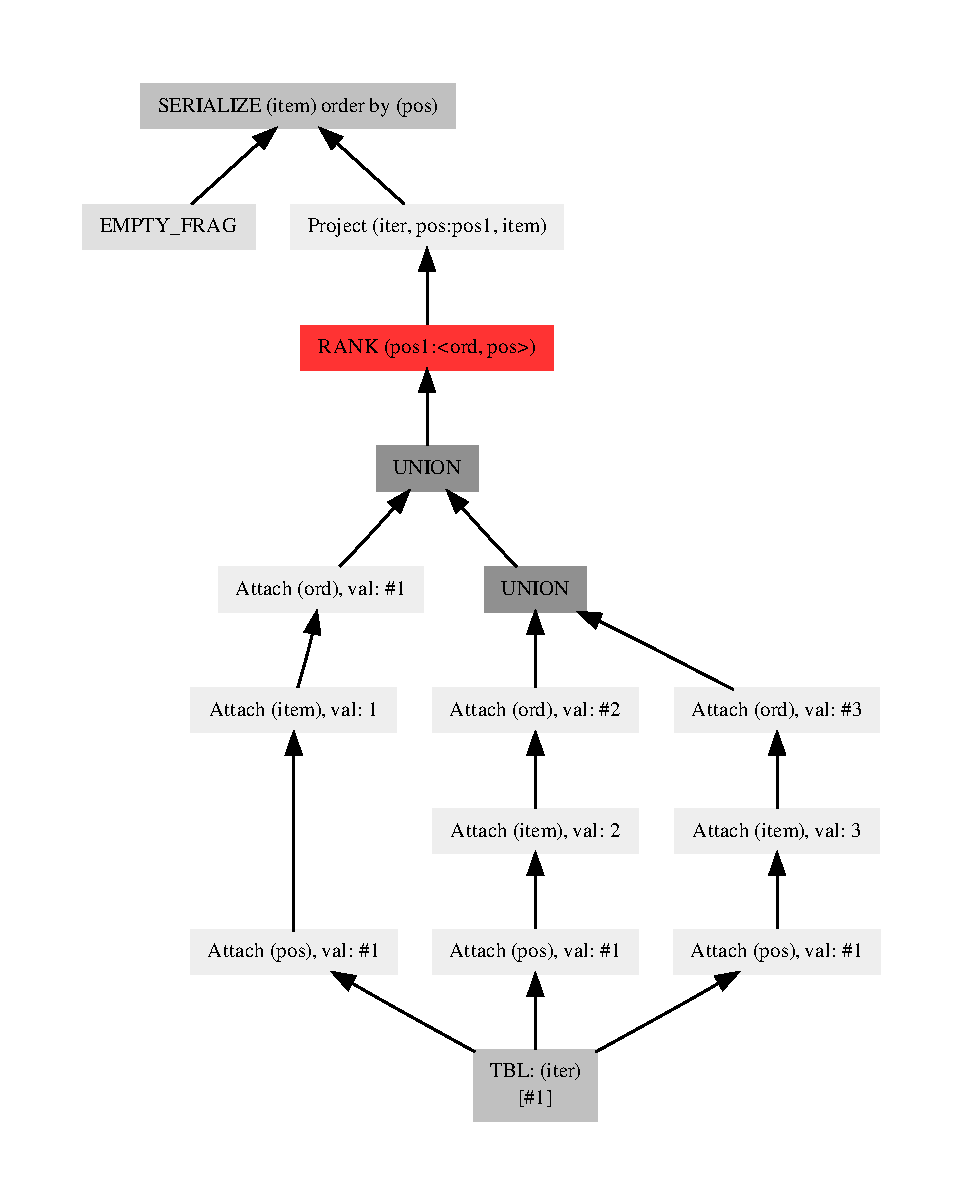
\includegraphics[width=0.4\textwidth]{img/graphs/td_impl_flwor_simple_pathfinder}
			\label{fig:result:comparison:simple_dag}
		}
		\quad
		\subfigure[Prototype implementation]{
		
			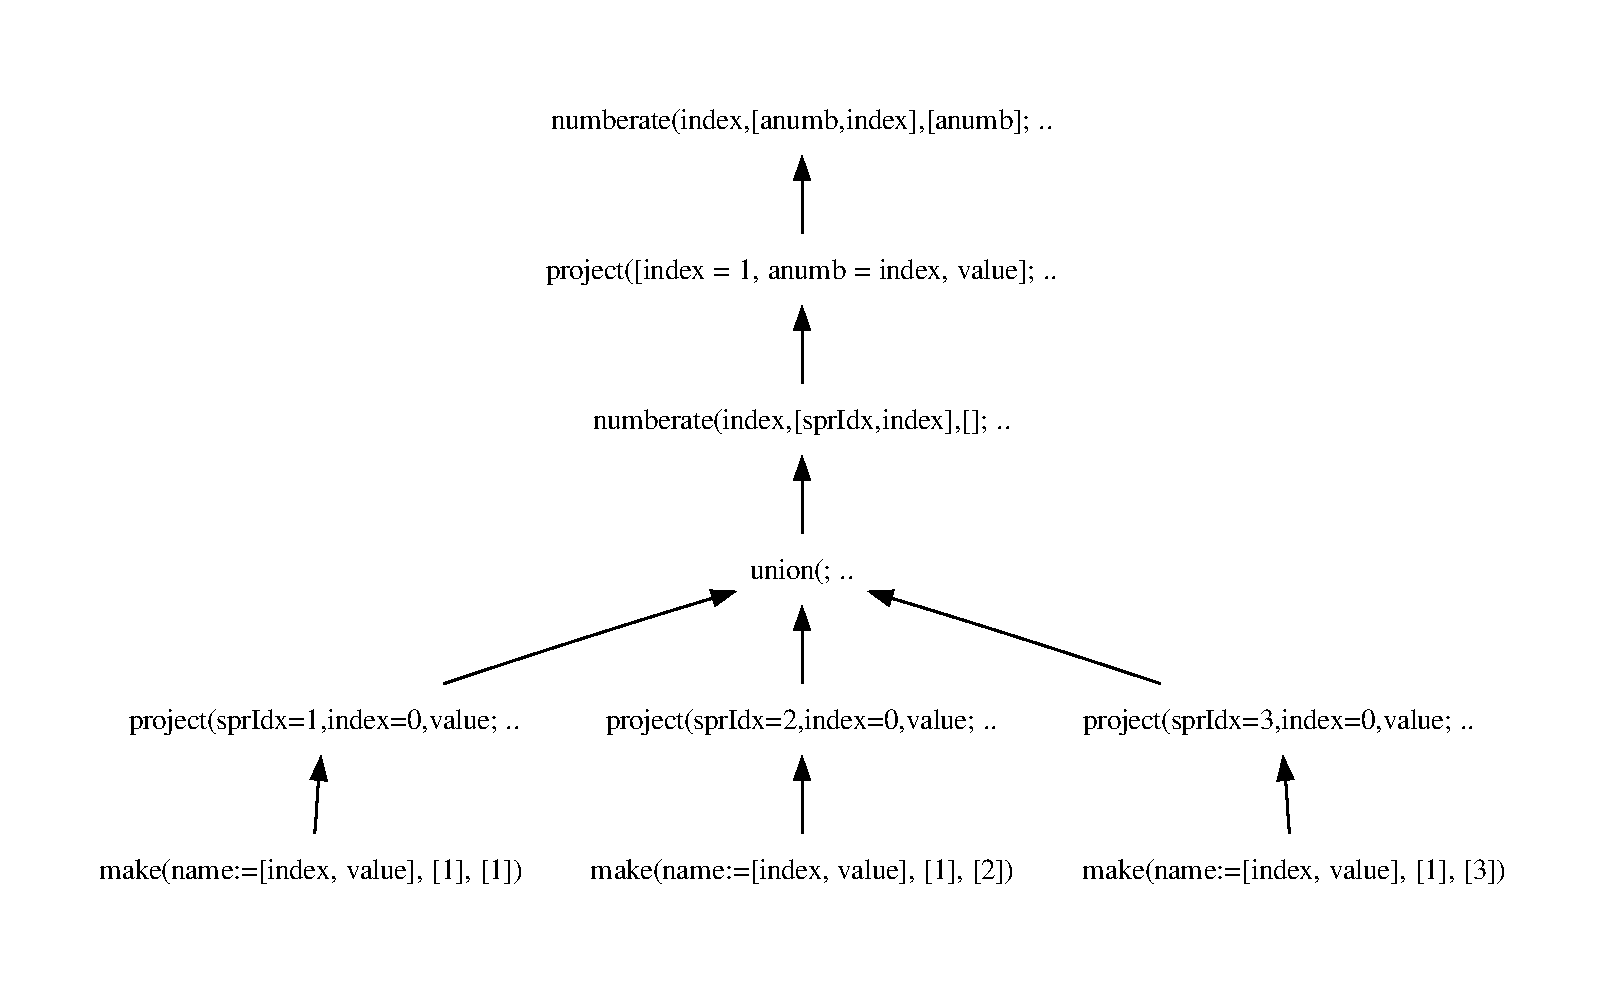
\includegraphics[width=0.6\textwidth]{img/graphs/td_impl_flwor_simple_xq_relalg}
			\label{fig:result:comparison:simple_pathfinder_dag}
		}
	}
	\caption{Comparison of DAGs for the trivial expression in section
	\ref{sect:results:algebra:generated:trivial_flwor}}
\end{figure}

\newpage
\begin{figure}[!h]
	\centering
	\mbox{
		\subfigure[Pathfinder/MonetDB]{		
			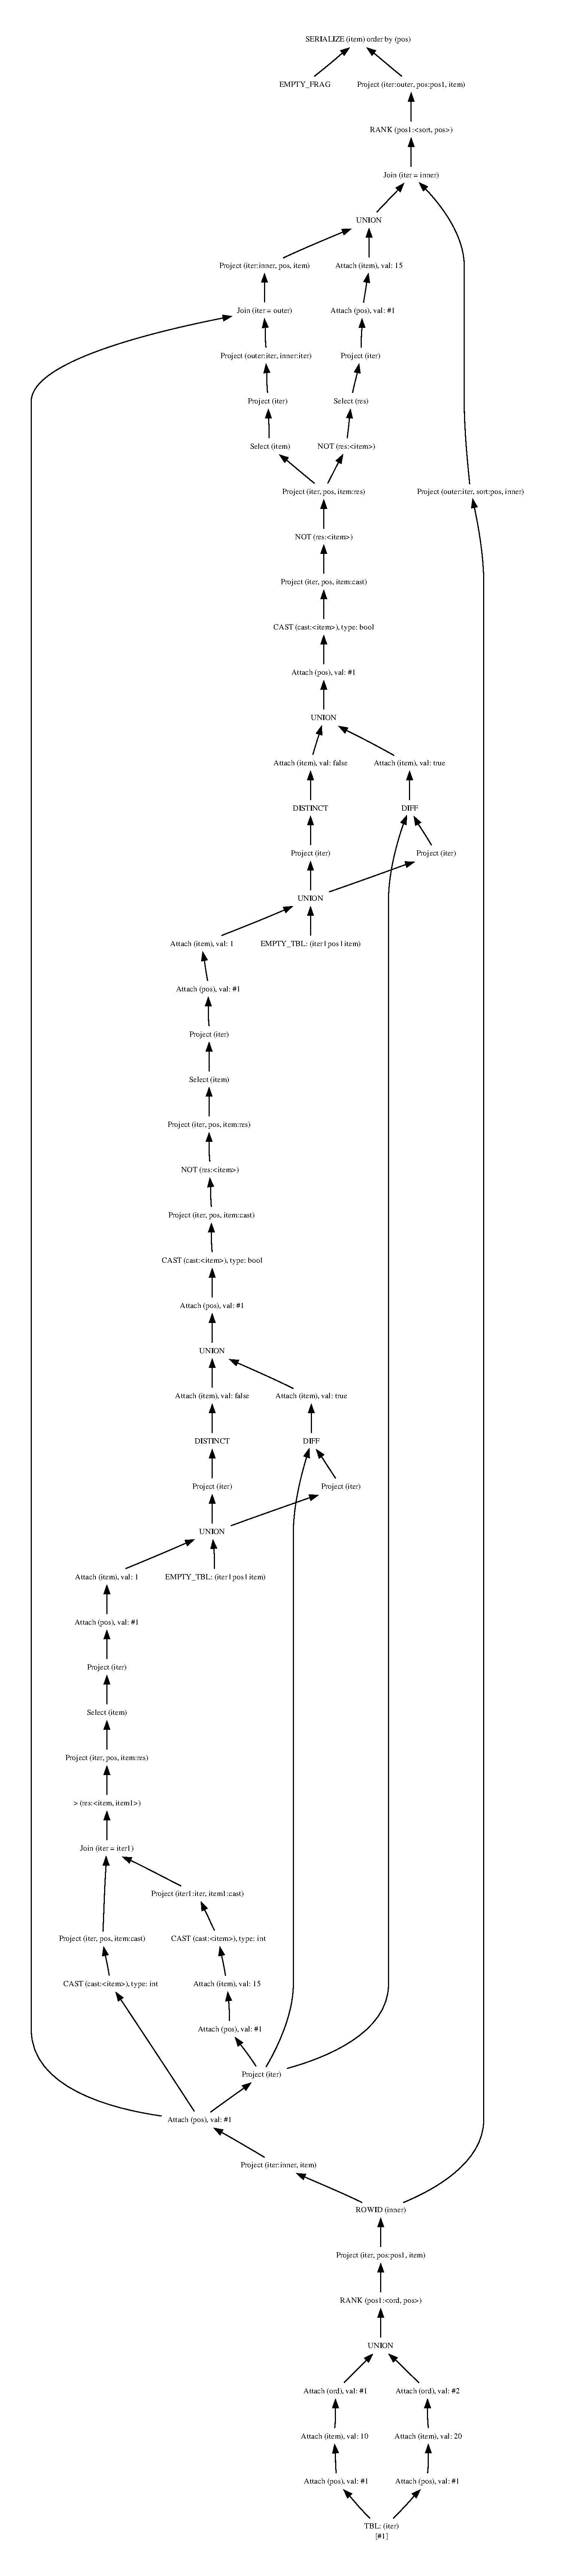
\includegraphics[width=0.3\textwidth]{img/graphs/td_impl_flwor_ifthenelse_pathfinder}
			\label{fig:result:comparison:conditional_dag}
		}
		\quad
		\subfigure[Prototype implementation]{
		
			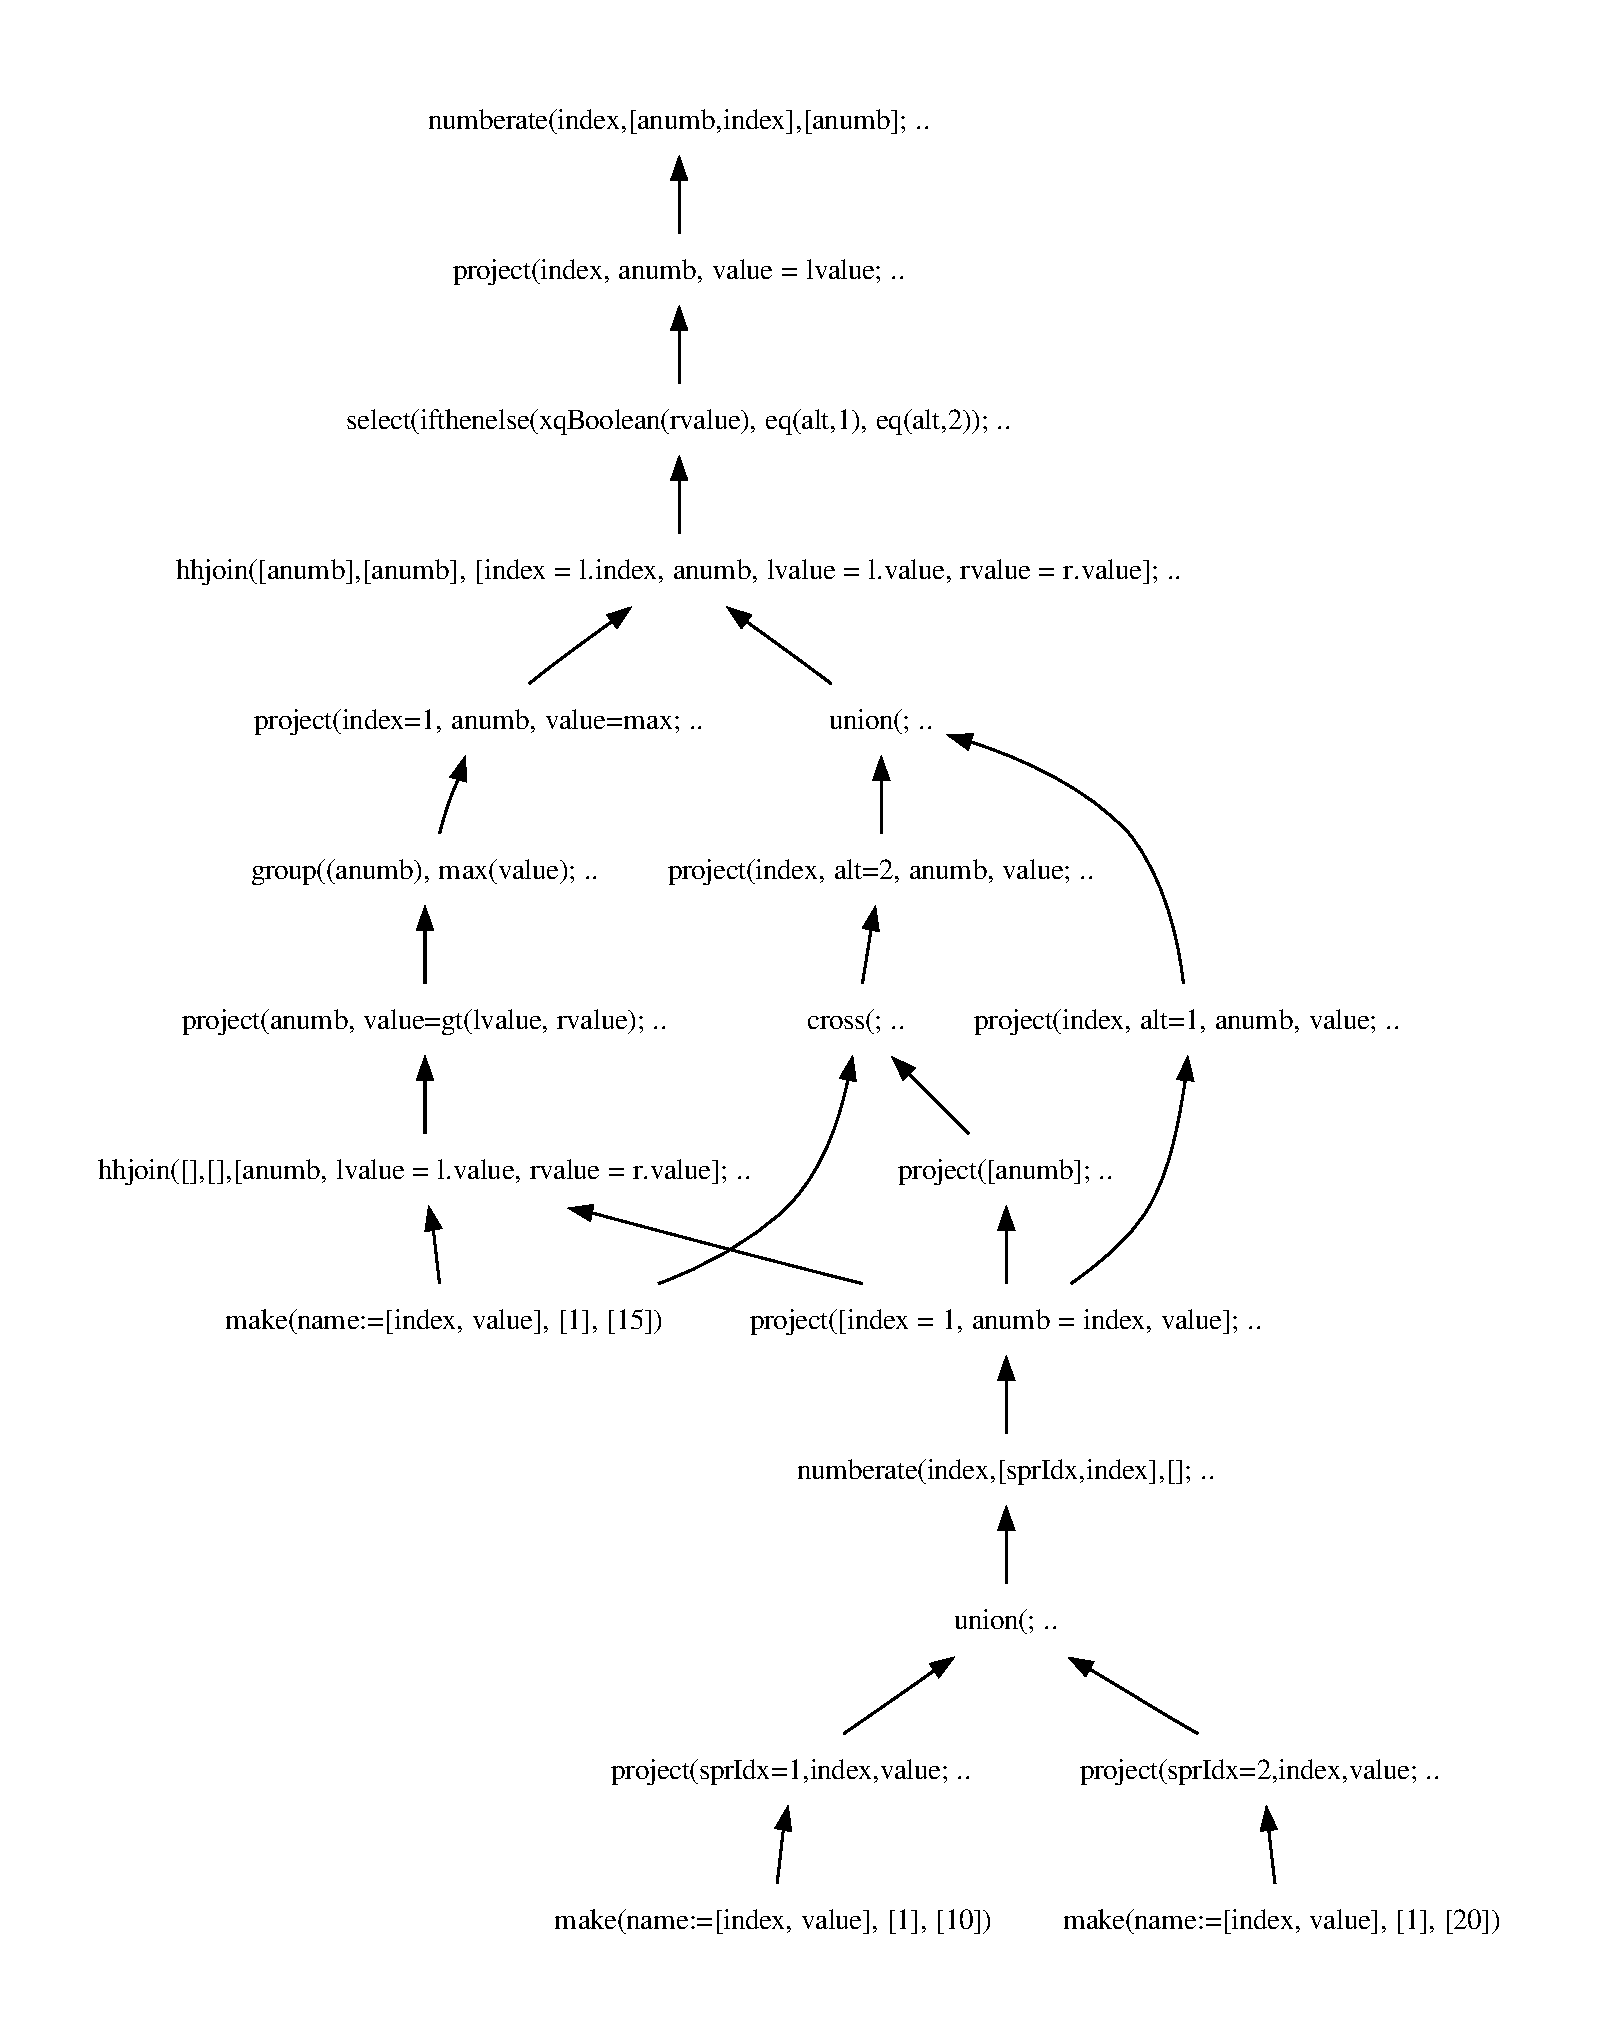
\includegraphics[width=0.7\textwidth]{img/graphs/td_impl_flwor_ifthenelse_xq_relalg_dag}
			\label{fig:result:comparison:conditional_pathfinder_dag}
		}
	}
	\caption{Comparison of DAGs for the conditional expression in section
	\ref{sect:results:algebra:generated:conditional_flwor}}
\end{figure}

\newpage
\begin{figure}[!h]
	\centering
	\mbox{
		\subfigure[Pathfinder/MonetDB]{		
			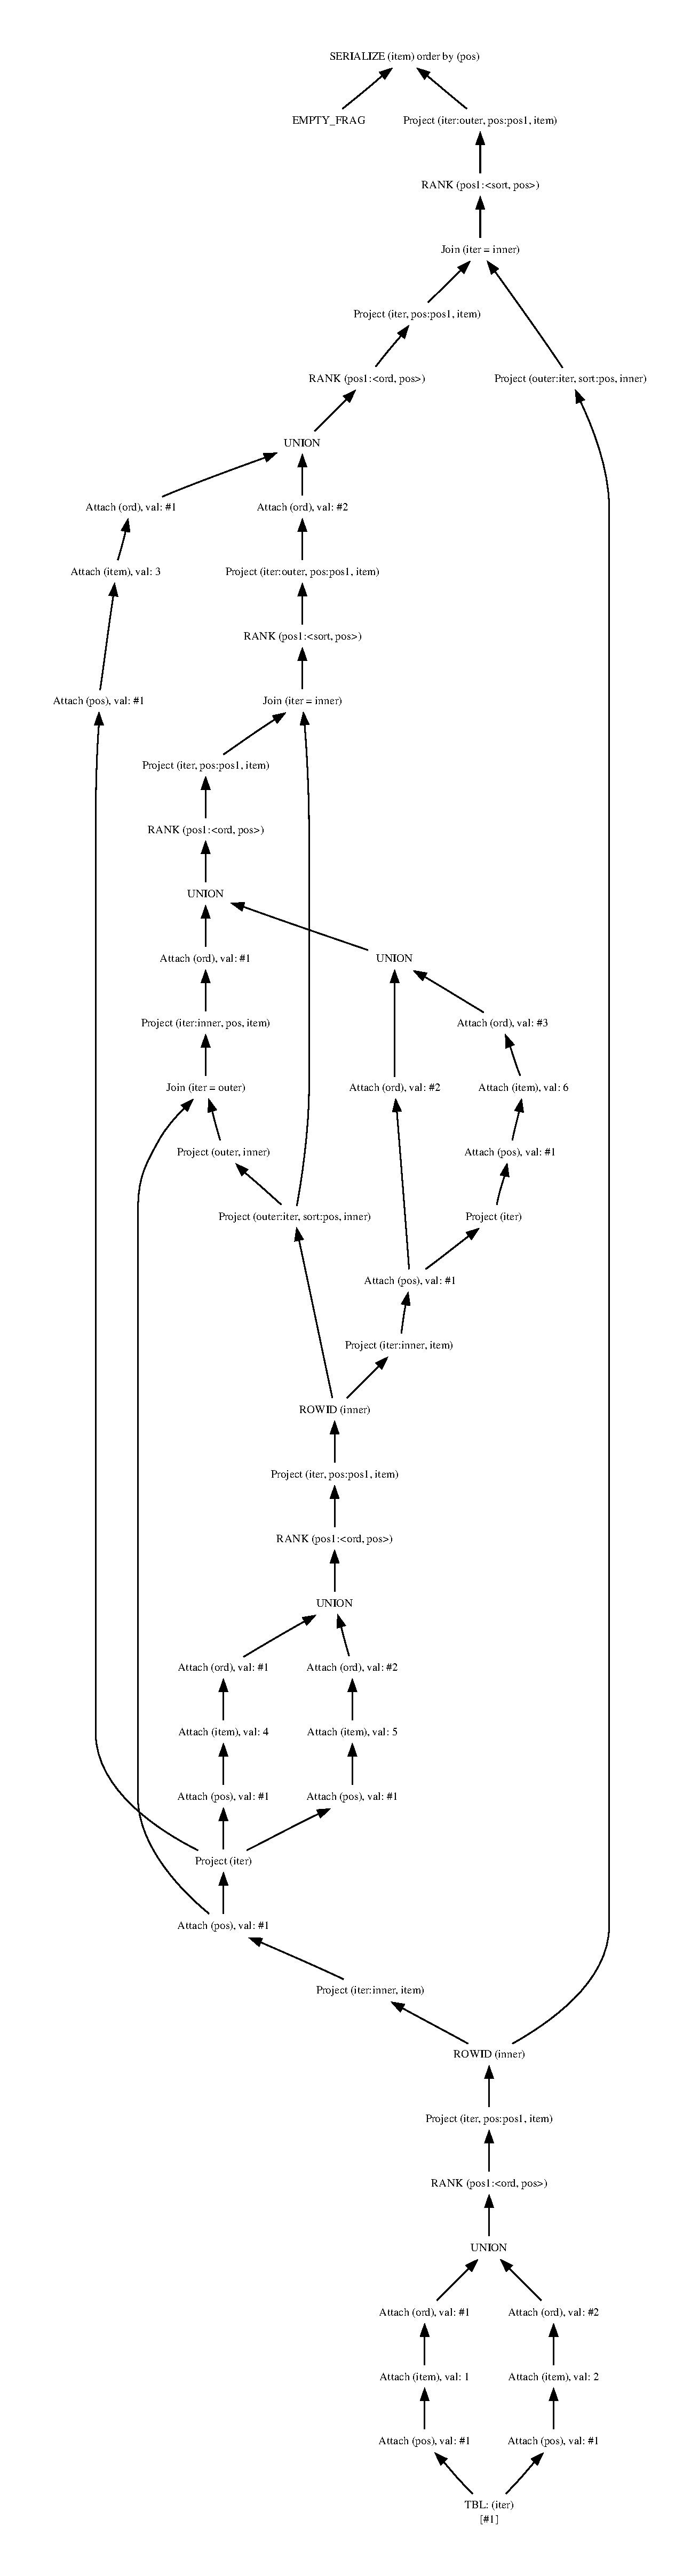
\includegraphics[width=0.37\textwidth]{img/graphs/td_impl_flwor_complex_pathfinder}
			\label{fig:result:comparison:complex_xqft_dag}
		}
		\quad
		\subfigure[Prototype implementation]{
		
			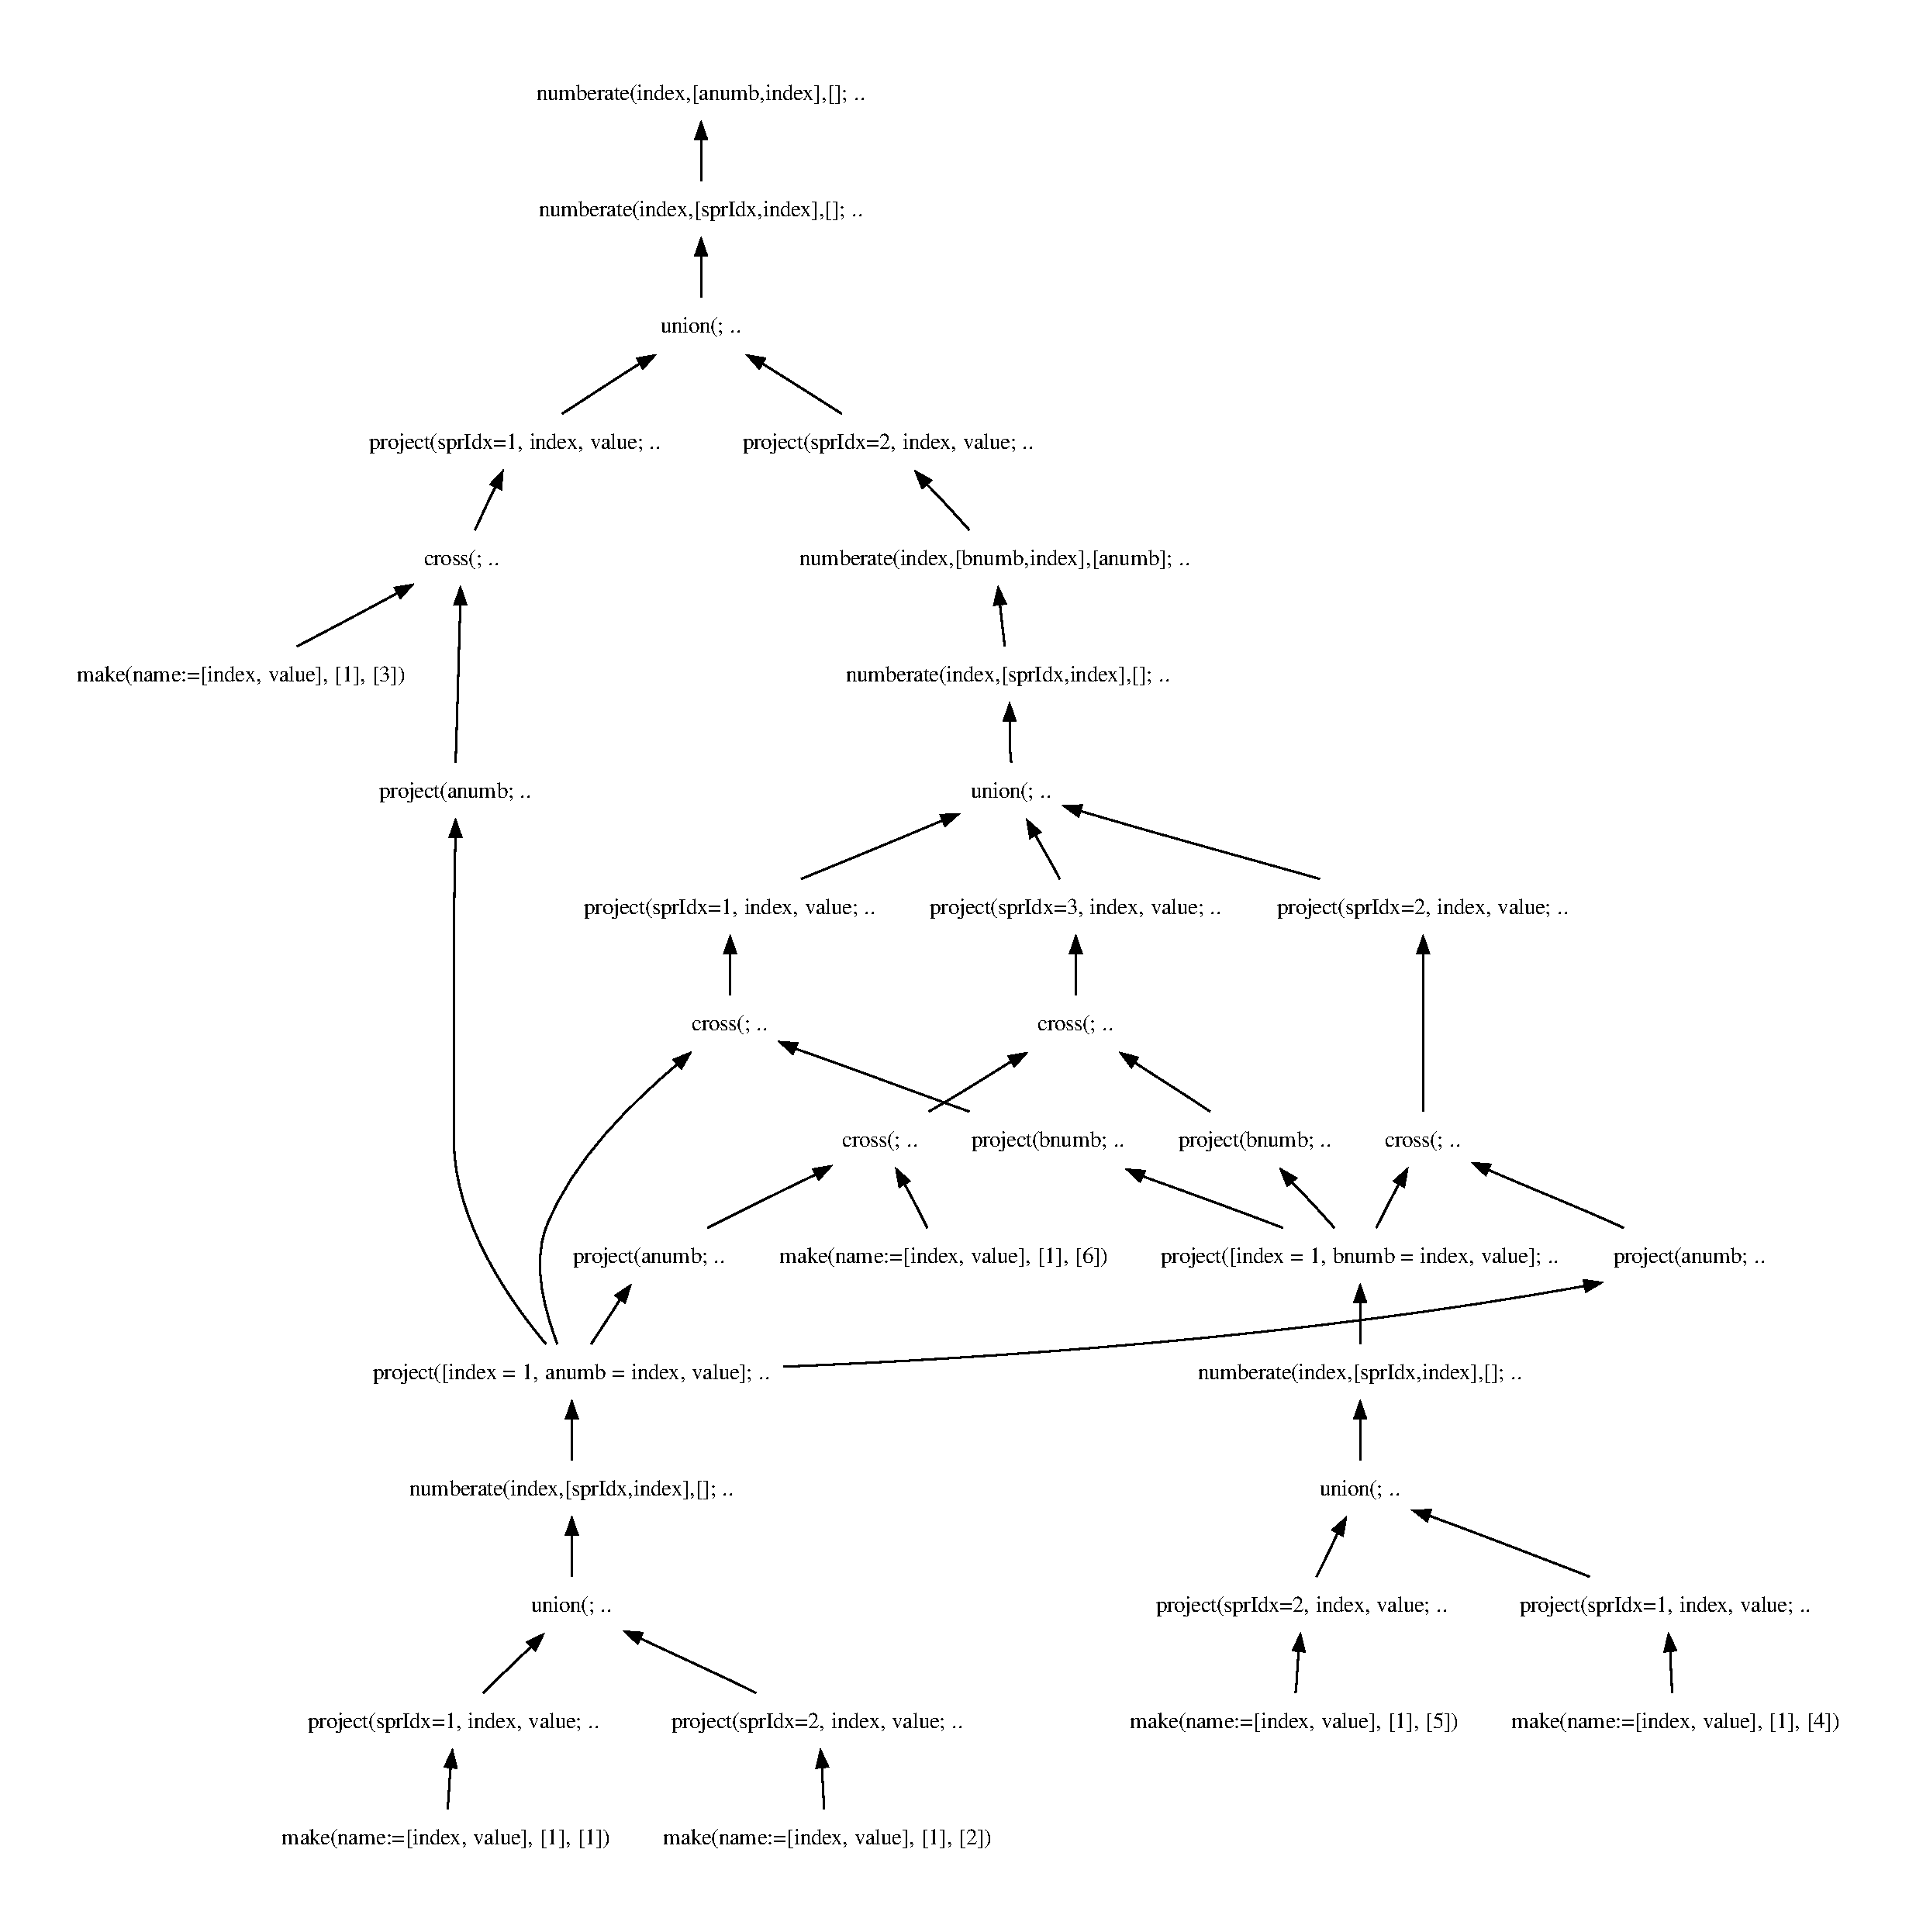
\includegraphics[width=0.6\textwidth]{img/graphs/td_impl_flwor_complex_xq_relalg_dag}
			\label{fig:result:comparison:complex_pathfinder_dag}
		}
	}
	\caption{Comparison of DAGs for the complex expression in section
	\ref{sect:results:algebra:generated:complex_flwor}}
\end{figure}

\newpage
\subsection{Complexity estimation and comparison}
Complexity estimation is performed as detailed in section
\ref{sect:method:complexity}. The complexity
comparison matrix is shown in table \ref{table:result:complexity_matrix}.

\begin{table}[!htp]
 \begin{center} 
 \begin{tabular}{| c | c | c || c | c |}
  \hline
   & \multicolumn{2}{|c||}{\textbf{Pathfinder/MonetDB}}
   & \multicolumn{2}{|c|}{\textbf{Prototype implementation}} \\
   \hline
   & Tuples & Fields & Tuples & Fields \\  
   \hline
   Trivial & 16 & 16 & 15 & 18 \\  
   \hline
   Complex & 215 & 265 & 136 & 102 \\
   \hline
   Conditional & 94 & 50 & 31 & 44 \\  
   \hline
 \end{tabular}
\caption{Complexity comparison matrix}
\label{table:result:complexity_matrix}
 \end{center}
\end{table}




\begin{figure}[!htp]
\begin{center}
  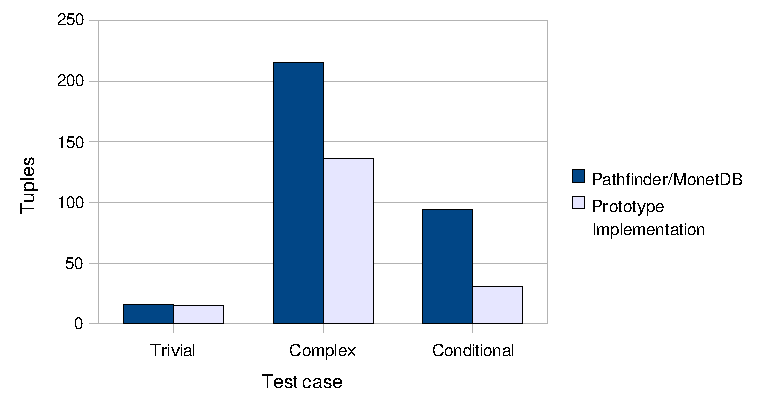
\includegraphics[width=1.0\textwidth]{diagrams/comparison_chart2_chart1}
  \caption{Comparison of complexity based on tuple creation}
  \label{fig:results:comparison:chart1}
\end{center}
\end{figure}

\begin{figure}[!htp]
\begin{center}
  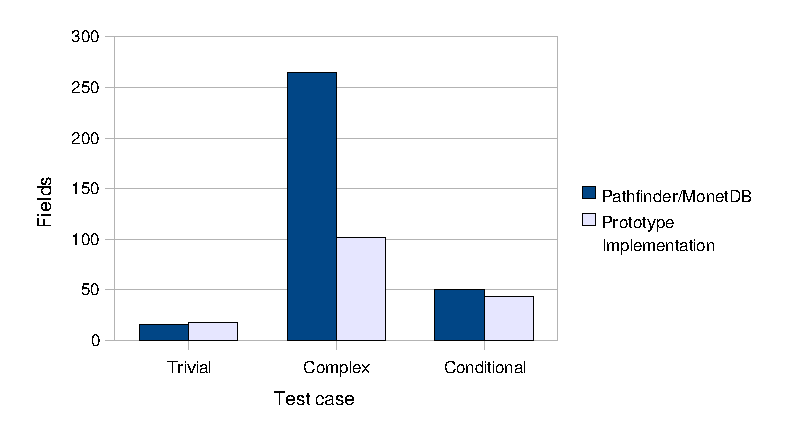
\includegraphics[width=1.0\textwidth]{diagrams/comparison_chart2_chart2}
  \caption{Comparison of complexity based on field creation}
  \label{fig:results:comparison:chart2}
\end{center}
\end{figure}

% Joins
\begin{table}[!htp]
 \begin{center}
 \begin{tabular}{| c | c | c | c | c | c | c | c |}
  \hline
   & \multicolumn{7}{|c|}{\textbf{Pathfinder}} \\
   \hline
   &  & \multicolumn{3}{|c|}{\textbf{In}} &
   \multicolumn{3}{|c|}{\textbf{Out}}  \\
   \hline
   &  \# & Min & Max & Avg & Min & Max & Avg\\
   \hline
   Trivial & 0 & 0 & 0 & 0 & 0 & 0 & 0  \\
   \hline
   Complex & 3 & 6 & 14 & 12.67 & 4 & 14 & 10  \\
   \hline
   Conditional & 3 & 4 & 6 & 4.67 & 1 & 2 & 1.67  \\
   \hline
   %\hline
   & \multicolumn{7}{|c|}{\textbf{Prototype}} \\
   \hline
   &  & \multicolumn{3}{|c|}{\textbf{In}} & 
   \multicolumn{3}{|c|}{\textbf{Out}} \\
   \hline
   & \# & Min & Max & Avg & Min & Max & Avg \\ 
   \hline 
   Trivial & 0 & 0 & 0 & 0 & 0 & 0 & 0 \\
   \hline
   Complex & 0 & 0 & 0 & 0 & 0 & 0 & 0 \\
   \hline
   Conditional & 2 & 3 & 6 & 4.5 & 3 & 6 & 4.5 \\
   \hline
 \end{tabular}
\caption{Tuple input/output in join operators}
\label{table:result:complexity_matrix}
 \end{center}
\end{table}


% Sorts
\begin{table}[!htp]
 \begin{center}
 \begin{tabular}{| c | c | c | c | c | c | c | c |}
  \hline
   & \multicolumn{7}{|c|}{\textbf{Pathfinder}} \\
   \hline
   &  & \multicolumn{3}{|c|}{\textbf{In}} &
   \multicolumn{3}{|c|}{\textbf{Out}}  \\
   \hline
   &  \# & Min & Max & Avg & Min & Max & Avg\\
   \hline
   Trivial & 1 & 3 & 3 & 3 & 3 & 3 & 3  \\
   \hline
   Complex & 6 & 2 & 14 & 8.8 & 2 & 14 & 8.8  \\
   \hline
   Conditional & 2 & 2 & 2 & 2 & 2 & 2 & 2  \\
   \hline
   %\hline
   & \multicolumn{7}{|c|}{\textbf{Prototype}} \\
   \hline
   &  & \multicolumn{3}{|c|}{\textbf{In}} &
   \multicolumn{3}{|c|}{\textbf{Out}} \\
   \hline
   & \# & Min & Max & Avg & Min & Max & Avg \\
   \hline
   Trivial & 2 & 3 & 3 & 3 & 3 & 3 & 3 \\
   \hline
   Complex & 6 & 2 & 14 & 9.33 & 2 & 14 & 9.33 \\
   \hline
   Conditional & 2 & 2 & 2 & 2 & 2 & 2 & 2 \\
   \hline
 \end{tabular}
\caption{Tuple input/output in join operators}
\label{table:result:complexity_matrix}
 \end{center}
\end{table}

\section{Summary}
\label{sect:res:summary}
In this chapter, a series of algebra trees have been presented. To diversify,
algebra computed by hand as well as algebra generated by the prototype
implementation has been presented. 

In the next chapter, these results as well as challenges and problems are
discussed in detail.
